\documentclass[11pt]{article}
\usepackage[english]{babel}
\usepackage[utf8]{inputenc}
\usepackage[T1]{fontenc}
\usepackage{float}
\usepackage{lmodern,amsmath,amssymb,amstext,amsfonts,mathrsfs,graphicx,caption, subcaption}
\usepackage[width=14cm]{geometry}
\usepackage[colorlinks,pdfpagelabels,pdfstartview = FitV,bookmarksnumbered = true, bookmarksopenlevel=section, linkcolor = black,hypertexnames = false,citecolor = black,pdfpagelabels=false]{hyperref}
\usepackage{tablefootnote}
%\usepackage{rotating}
\usepackage{textcmds, enumitem}
\usepackage{sidecap} %, indentfirst
\usepackage[labelfont={bf,sf},font={small},labelsep=space]{caption}
\usepackage{chngcntr} % 			** Damit die Bilder Tabellen und Gleichungen 
\counterwithin{figure}{section}	%	** alle nach Kapiteln nummeriert sind.
\counterwithin{table}{section}%		**
\counterwithin{equation}{section}%	**	

\begin{document}
	\section{Results}
	
	\subsection{The Correlation between Response Properties from symmetrical Recurrent Interaction Networks and Feedforward Recurrent Alignment} \label{sec:results_symmetric}
	% TODO: is inspired by the Rayleigh Coefficient for eigenvalue approximation in mathmatics. -- literature to it. 
	The feedforward recurrent alignment, defined in the method under section \ref{sec:ffrec_definition} quantifies the degree of how much the feedforward input is aligned with the direction that is spanned by eigenvectors of the recurrent network. If the input is well aligned with the eigenvector corresponding to the maximal eigenvalue of the recurrent interaction $J$, the random noise in the response would be suppressed by the evoked response due to selective amplification. Response amplification determines the steady-state response, 
		\begin{equation} \label{eq:response_amplification}
			r^* = \sum_{i = 1}^{n} \frac{(e_i \cdot h) e_i}{1-\lambda_i} \, ,
		\end{equation}
	where $\cdot$ denotes the dot product between two vectors. 
	
	The steady state response is then dominated by the projection of the input vector $h$ along the axis defined by the eigenvector $e_{\text{max}}$ whose eigenvalue $\lambda_{\text{max}}$ is maximal and near one \cite{dayan2005theoretical}. 
		\begin{equation} \label{eq:selective_amplification}
			r^* \approx \frac{(e_{\text{max}} \cdot h) e_{\text{max}}}{1 - \lambda_{\text{max}}}
		\end{equation}
	The projection of input $h$ on eigenvector $e_{\text{max}}$ reaches its maximal when $h$ is approximately $e_{\text{max}}$ itself. Therefore, the steady state responses reaches its maximum and the feedforward recurrent alignment equals the maximal eigenvalue $\lambda_{\text{max}}$ of $J$ because of eq.(\ref{eq:ffrec_equals_eigval}). 
	
	On the other hand, if the input is not well aligned with the dominant eigenvectors, the random noise is large relative to the response. For an extreme example, if the input is aligned with the eigenvector $e_{\text{min}}$ with minimal eigenvalue $\lambda_{\text{min}}$, the response will almost not contribute to the steady state response at all due to the response amplification eq.(\ref{eq:response_amplification}). This could also be reflected by the feedforward recurrent alignment, which equals $\lambda_{\text{min}}$ in this case because of eq.(\ref{eq:ffrec_equals_eigval}). 
	
	We can thus conclude that the feedforward recurrent alignment eq.(\ref{eq:ffrec_align}) reflects the alignment between the feedforward input and the dominant eigenvectors of the recurrent interaction network $J$. The better the input $h$ is aligned to the dominant eigenvectors of $J$, the stronger and more reliable the response, and at the same time the higher the feedforward recurrent alignment score.
	
	In the following sections, the four properties introduced at section \ref{sec:response_properties_for_evaluation} will be evaluated in the model and compare to the tendency observed in \cite{tragenap2023nature}. 
	
	\subsubsection{Trial-to-Trial Correlation increases with larger Alignment}
	
	As defined under section \ref{sec:response_properties_for_evaluation} in paragraph "Trial-to-trial correlation", the inputs are constructed by multivariate normal distribution eq.(\ref{eq:input_distribution}). When aligning the input $h$ with eigenvectors $e_i$, $e_i$ are the the mean vector for input distribution as defined in eq.(\ref{eq:input_distribution}), 
		\begin{equation}
			h_i \sim \mathcal{N} (e_i, \sigma_{\text{trial}}^2 I_n) \, . 
		\end{equation}
	The feedforward recurrent alignment score is then determined by corresponding eigenvalue $\lambda_i$ due to eq.(\ref{eq:ffrec_equals_eigval}), and reaches its maximal when align input $h$ to $e_{\text{max}}$. 
	%The degree of alignment of input on the dominant eigenvector $e_{\text{max}}$ is then determined approximately by the size of eigenvalue, to which the eigenvector is corresponded. 
	
	%And as explained above, the better the input is aligned with the dominant eigenvector, the better the approximation. 
	
	We want to find out the correlation between the feedforward recurrent and the trial-to-trial correlation $\beta_s$ defined by eq.(\ref{eq:ttc_sym}). If sorting the eigenvectors in the order such that their corresponding eigenvalues are in ascending order, 
		\begin{equation} \label{eq:ascending_order}
			e_{\text{min}}, ..., e_i, e_j, ..., e_{\text{max}} \, \, \text{such that} \, \, \lambda_{\text{min}} < ...< \lambda_i < \lambda_j < ... < \lambda_{\text{max}} \, ,
		\end{equation}
	with $\lambda_i$ the corresponding eigenvalue for eigenvector $e_i$. The inputs that aligned with eigenvectors in this order should have monotonously increasing feedforward recurrent alignments.
	
	Generating the results with eq.(\ref{eq:steady_state_distribute}) for $N$ trials. The trial-to-trial correlation can be calculated with eq.(\ref{eq:ttc_sym}). 

		\begin{SCfigure}[0.9][h] 
			\centering
			\caption[Correlation between feedforward recurrent alignment and trial-to-trial correlation for symmetric RNNs]{\textbf{Correlation between feedforward recurrent alignment and trial-to-trial correlation for symmetric RNNs.} Inputs aligned to eigenvectors $e_i$ of interaction matrix $J$ in the ascending order of eigenvalues eq.(\ref{eq:ascending_order}), resulting the feedforward recurrent alignment varies approximately between $\lambda_{\text{min}}$ and $\lambda_{\text{max}}$. For each input alignment to an eigenvector, $N=100$ trials of evoked responses were generated for calculation of the trial-to-trial correlation calculated with eq.(\ref{eq:ttc_sym}).}
			\includegraphics[width=0.5\textwidth]{../figures/ttc_sym(2).pdf}
			\label{fig:ttc_ffrec_sym}
		\end{SCfigure}
	
	We assume feedforward recurrent alignment for visually naive cortex equals zero, which could be interpreted as responses evoked by random inputs. The trial-to-trial correlation with random inputs is smaller than it in the case, when the input is aligned to $e_{\text{max}}$. This coincides with the experimental observations of responses from visually naive and experienced primary visual cortex of ferrets \cite{tragenap2023nature}. 
	
	Moreover, the modeling result Figure \ref{fig:ttc_ffrec_sym} suggests a positive correlation between the feedforward recurrent alignment and the trial-to-trial correlation over the whole alignment range. The result confirms the idea that with the feedforward inputs more and more aligned with the dominant eigenvectors of the recurrent network, the stability between trials increases also simultaneously. The process of reaching higher trial-to-trial stability is therefore a process of becoming more aligned with the dominant eigenvector. 
	This positive correlation also coincides with the experimental results from ferrets \cite{tragenap2023nature}.
	
	%The positive correlation between the feedforward recurrent alignment and the trial-to-trial correlation coincident with the experimental observations od responses from visually naive and experienced primary cortex of ferrets \cite{tragenap2023nature}. Moreover, the modulation suggests that 
	
	\subsubsection{Intra-Trial Stability increases with larger Alignment}
	
	Now we want to see if our modeling could capture the change in intra-trial stability during the development observed in the primary visual cortex of ferrets \cite{tragenap2023nature}. The intra-trial stability increased after the eye-opening and a couple of days. The feedforward recurrent alignment hypothesis suggests that the visually experienced cortex should have a better alignment between feedforward inputs and the dominant modes in the recurrent network. To confirm this idea, we would expect the intra-trial stability would be larger with a higher feedforward recurrent alignment score. 
	
	Analogous to trial-to-trial correlation, the eigenvectors can be sorted in descending order according to the eigenvalues eq.(\ref{eq:ascending_order}). The intra-trial stability is calculated with eq.(\ref{eq:its_sym}).

	\begin{SCfigure}[0.9][h] 
		\centering
		\caption[Correlation between feedforward recurrent alignment and intra-trial stability for symmetric RNNs]{\textbf{Correlation between feedforward recurrent alignment and intra-trial stability for symmetric RNNs.} Inputs aligned to eigenvectors $e_i$ of interaction matrix $J$ sorted according to the ascending order of eigenvalues eq.(\ref{eq:ascending_order}), resulting the feedforward recurrent alignment varies approximately between $\lambda_{\text{min}}$ and $\lambda_{\text{max}}$. For one input aligned to an eigenvector, the intra-trial stability is calculated with the evoked steady-state response eq.(\ref{eq:its_sym}).}
		\includegraphics[width=0.5\textwidth]{../figures/its_sym(2).pdf}
		\label{fig:its_ffrec_sym}
	\end{SCfigure}

	The result (Figure \ref{fig:its_ffrec_sym}) indicates a positive correlation between the feedforward recurrent alignment and the intra-trial stability. With random feedforward inputs, the feedforward recurrent alignment takes the value near zero. So the eye-opening happens somewhere between feedforward recurrent equals zero and reaches maximal. Thus, before the eye-opening, there is already a certain alignment that leads to a certain degree of intra-trial correlation. 
	
	Furthermore, the correlation is almost exponential. So, the enhancement of the input alignment to the dominant eigenvector is more rapid after the eye-opening than before. One assumption for this phenomenon could be that after the eye-opening, the environment provides more training data for the network so that the alignment between inputs and the dominant eigenvector could be improved more efficiently. As a result, the responses get more intense and drive a better alignment forward. A positive loop could arise and speed up until the optimum is reached. 
	
	\subsubsection{Dimensionality decreases with larger Alignment}
	
	Dimensionality is a generally important property of neural representations and could help to understand processes for example in learning and controlling \cite{bartolo2020dimensionality, badre2021dimensionality}. A low-dimensional representation will encode a diverse range of inputs into a small set of common, orthogonal activity patterns. In other words, low-dimensional activity patterns require a small number of basis vectors from the response space to represent themselves. On the contrary, a high-dimensional representation will separate even similar inputs into orthogonal activity patterns. Compared to low-dimensional representation, a high-dimensional activity pattern is represented through a large set of basis vectors \cite{badre2021dimensionality}. 
	
	Therefore, we want to take a look at the change of dimensionality during the increase of alignment in the modeling. In ferrets' primary visual cortex, the dimensionality decreased from days before eye opening until days after eye-opening \cite{tragenap2023nature}. We would then expect that the model should also suggest a decrease in dimensionality with an increase in alignment between inputs and dominant eigenvectors of recurrent networks. 
	
	For a certain alignment, the principal component analysis reflects directly the dimensionality of the evoked activity pattern under this alignment. Because the principal components are the eigenvectors of response covariance, they also build up a set of basis vectors for the activity pattern space. Variance ratios reflect the weight that each principal component takes to represent the activity pattern. Thus, if only a small number of principal components contribute the most, the activity pattern is then low dimensional. If a broad set of principal components are similarly important, the activity pattern is highly dimensional.  
	
	With the idea of obtaining the linear dimensionality defined as participation ratio 
	%TODO: \cite{abbott2011interactions}  
	based on the principal component analysis, the eigenvectors here are ordered in descending order, 
		\begin{equation} \label{eq:descding_order}
			e_{\text{max}}, ..., e_i, e_j, ..., e_{\text{min}} \, \, \text{such that} \, \, \lambda_{\text{max}} > ...> \lambda_i > \lambda_j > ... > \lambda_{\text{min}} \, .
		\end{equation}
	%For the calculation of the linear dimensionality (\ref{eq:dim_analytical_sym}) and (\ref{eq:dim_empirical_sym}), 
	For the generation of inputs with covariance matrix $\Sigma^{\text{Dim}}$ defined in eq.(\ref{eq:Sigma_dim}), a subset of eigenvectors $\{e_i\}_{i = L, ..., L+M_{\text{dim}}}$ will be chosen for $L=1, ..., \frac{n}{2}$. $M_{\text{dim}}$ then determines how many eigenvectors will contribute to generating inputs and evoked activity. In each such subset of eigenvectors, the leading eigenvector is $e_L$. Approximate here the feedforward recurrent alignment with the leading eigenvector only. Since $L$ is considered only in the range of the first half of eigenvectors ordered as eq.(\ref{eq:descding_order}), the range of feedforward recurrent alignment is between around $0$ and $\lambda_{\text{max}}$. The linear dimensionality analytically and empirically will be calculated according to eq.(\ref{eq:dim_analytical_sym}) and eq.(\ref{eq:dim_empirical_sym}). 

		\begin{figure}[H] 
			\centering
			\begin{subfigure}[b]{0.45\textwidth} 
				\includegraphics[width=\textwidth]{../figures/dim_align_rand_sym(2).pdf}
				\caption{}
			\end{subfigure}
			\hfill
			\begin{subfigure}[b]{0.44\textwidth}
				\includegraphics[width=\textwidth]{../figures/dim_sym(2).pdf}
				\caption{}
				\label{fig:dim_sym}
			\end{subfigure}
			\vspace{-0.2cm}
			\caption[The correlation between dimensionality and feedforward recurrent alignment for symmetric RNNs]{\textbf{The correlation between dimensionality and feedforward recurrent alignment for symmetric RNNs.} Prior experimental observations suggested that the dimensionality decreases from prior until post eye-opening \cite{tragenap2023nature}. With the feedforward recurrent alignment hypothesis, the dimensionality property of the neural representation during development could be captured. \textbf{(a)} Principal component analysis for the evoked activity under input aligned to $e_{\text{max}}$ and spontaneous random activity. The red line is for maximal alignment and the green line is for spontaneous alignment. \textbf{(b)} Obtain the correlation between dimensionality and feedforward recurrent alignment with analytically eq.(\ref{eq:dim_analytical_sym}) and empirically eq.(\ref{eq:dim_empirical_sym}). The green line displays the analytical approximation for dimensionality and the blue dots for empirical.} 
			\label{fig:correlation_dim_ffrec_sym}
		\end{figure}

	As explained above, the principal component analysis helps to decode the dimensionality. The curve in Figure \ref{fig:correlation_dim_ffrec_sym}a of the variance ratio reflects the dimensionality. Spontaneous random alignment has a flatter variance ratio curve, indicating a broader range of eigenvector contributions. Therefore, the spontaneous random alignment has a higher dimensionality than under alignment with $e_{\text{max}}$. 
	%With the feedforward recurrent alignment hypothesis, the spontaneous random alignment matches the state before the eye opening and the maximal alignment for the state after eye opening. Therefore, the hypothesis results the same tendency of dimensionality decrease that observed in ferrets\cite{tragenap2023nature}.
	
	In total, a negative correlation between the dimensionality and feedforward recurrent alignment is shown in Figure \ref{fig:correlation_dim_ffrec_sym}b. The correlation forms nearly a flipped logarithmic function. The error between analytical and empirical results is small, which confirmed the good approximation formulated analytically by eq.(\ref{eq:dim_analytical_sym}). 
	
	Besides, the flipped logarithmic correlation suggests the a similar principle for intra-trial stability (Figure \ref{fig:correlation_dim_ffrec_sym}). After eye-opening, the reduction of dimensionality becomes larger when the feedforward inputs align better with the dominant eigenvector. It could be the case, that after the eye-opening, the recurrent network tries to encode the environment information with a large number of eigenvectors, which is costly for the system. After some time of getting used to the stimuli and the evoked activity becomes more stable, the information is more determined, and fewer eigenvectors are needed to efficiently to encode it.
	%the system speed up to find out a more efficient encoding with fewer eigenvectors and the information becomes more determined. 
	%After finding out a better solution, the improvement will be speed up until the optimum encoding with at least number of eigenvectors. 
	
	\subsubsection{Alignment to Spontaneous Activity Increases with larger Alignment}
	
	Spontaneous activity in neural systems is defined as neural activity that is not driven by an external stimulus. The activity patterns of spontaneous activity are not completely random and have often unique spatiotemporal patterns that instruct neural circuit development in the developing brain. Moreover, normal and aberrant patterns of spontaneous activity underline behavioral states and diseased conditions in adult brains. Therefore, spontaneous activity is essential for the understanding of brain development \cite{imaizumi2018spontaneous}. The alignment between activity patterns and spontaneous activity patterns could show the structural relation between patterns. %Besides, it could also reflect the presentation of spontaneous activity in other activity patterns. 
	
	In newborn ferrets' brains, visual responses that are loosely aligned with spontaneous activity in the cortex before eye-opening transformed to reliable and well-aligned responses several days after eye-opening \cite{tragenap2023nature}. Thus, we expect that the feedforward recurrent hypothesis can reflect the tendency that evoked activity aligned better with spontaneous activity during the development of the brain. 
	
	Under the assumption that at eye-opening, the patterns of feedforward inputs are aligned to random activity patterns, thus not as well aligned to the recurrent network as the spontaneous activity. The evoked and spontaneous pattern overlaps only a little (Figure \ref{fig:align_spont_act_sym}(a), visually comparing the green line to the red line.). It could be observed here that only the last few principal components have a similar variance ratio, while the first few dominant eigenvectors differ a lot. There is not much overlap between green and red curves. On the contrary, experience-driven changes that optimize the feedforward-recurrent alignment to $e_{\text{max}}$ results in a stronger overlap between distributions of evoked and spontaneous activity patterns (Figure \ref{fig:align_spont_act_sym}(a), visually comparing red line to blue line.). Most of the principal components have a similar explained variance ratio. The overlap between the red and blue line is significantly large. In both cases, the theoretical modeling hypothesis matches experimental observations in baby ferrets' brains \cite{tragenap2023nature}.
	
	To visualize and quantify the overlaps between activity patterns from evoked and endogenous patterns, we considered the summarized alignment score eq.(\ref{eq:align_to_spont_act_sym}). An exponential correlation between alignment to spontaneous activity and feedforward recurrent alignment (Figure \ref{fig:align_spont_act_sym}b) is suggested by the modeling. The strong growth of overlaps between evoked and endogenous activity starts only shortly before the optimal experience-driven alignment, indicating that the alignment could require a large amount of experience and training. The costly process of optimal alignment to spontaneous activity could on the other hand reflect the importance of the connection between evoked and endogenous activity patterns. 

		\begin{figure}
			\centering
			\begin{subfigure}[b]{0.44\textwidth} 
				\includegraphics[width=\textwidth]{../figures/align_to_spont_act_variance_ratio(2).pdf}
				\caption{}
				\label{fig:variance_ratio_sym}
			\end{subfigure}
			\hfill
			\begin{subfigure}[b]{0.45\textwidth}
				\includegraphics[width=\textwidth]{../figures/spont_align_ffrec_sym(2).pdf}
				\caption{}
				\label{fig:align_spont_sym}
			\end{subfigure}
			%\vspace{-0.1cm}
			\caption[Correlation between alignment to spontaneous activity and feedforward recurrent alignment score in symmetric RNNs]{\textbf{Correlation between alignment to spontaneous activity and feedforward recurrent alignment score in symmetric RNNs.} The spontaneous activity reflects inputs from a wide range of different sources and is considered to be already aligned to the recurrent network\cite{tragenap2023nature}. Aligning activity patterns to spontaneous activity is in principle to explain the activity pattern by the principal components of spontaneous activity. \textbf{(a)} Variance ratio eq.(\ref{eq:var_explain_spont_act_sym}) of spontaneous activity, evoked activity by feedforward input maximally aligned to recurrent network, and evoked activity by randomly aligned to recurrent network explained by principal components of spontaneous activity. The red line illustrates the variance ratio of spontaneous activity, the blue line the maximal alignment, and the green line the random alignment. Shadow shows the 95\% confidence interval for 50 symmetric RNNs. \textbf{(b)} The correlation between final alignment to spontaneous activity and feedforward recurrent alignment eq.(\ref{eq:align_to_spont_act_sym}). The eigenvalues are ordered in descending order as eq.(\ref{eq:descding_order}). Only the first half of eigenvectors are taken into account to determine the correlation.}
			\label{fig:align_spont_act_sym}
		\end{figure}

	
	\clearpage
	\subsection{Evaluation of Feedforward Recurrent Alignment Modulations for asymmetric Recurrent Interaction Networks} \label{sec:asymmetric_results}
	For symmetric interaction networks, the feedforward recurrent alignment hypothesis and the modeling based on it in section \ref{sec:results_symmetric} can demonstrate the response properties observed in ferrets \cite{tragenap2023nature}. With better alignment between inputs and recurrent network, key results of the response properties were
		\begin{itemize}
			\item The trial-to-trial correlation increases.
			\item The intra-trial stability increases.
			\item The Dimensionality decreases.
			\item The alignment of evoked activity to spontaneous activity increases.
		\end{itemize}
	
	However, since the symmetric interaction matrices simplify the neural connection dramatically, we try to embed the more biology-realistic asymmetric interaction matrices. Considering the modifications listed in methods in section \ref{sec:modify_ffrec_alignment_score}, we want to evaluate the modifications of the feedforward recurrent alignment score based on the key results we got with symmetric RNNs. 
	
	Firstly, we check if the feedforward recurrent alignment score keeps the proportionality to eigenvalues. We expect that a suitable modification could keep the monotonously positive correlation with eigenvalues. Then, we go through the four response properties to verify if the tendency above is still kept with increased alignment between inputs and recurrent network. 
	\vspace{0.5cm}
	\subsubsection{Monotony of Feedforward Recurrent Alignment Score in dependence of Eigenvalues}
	
	During the development, suggested by the feedforward recurrent alignment hypothesis for symmetric interactions, the inputs align better to the RNNs through aligning to dominant eigenvectors. Feedforward recurrent alignment is proportional to the corresponding eigenvalue of the eigenvector that is aligned with input eq.(\ref{eq:ffrec_equals_eigval}). 
	
	When considering the asymmetric interaction network, keeping the hypothesis that the inputs align more and more to the eigenvector with maximal eigenvalue, we examine if the modified feedforward recurrent alignment score could still keep the proportionality to eigenvalues. 
	%\footnote{Order the complex eigenvalues of the asymmetric interaction matrix through comparing the real parts. Undertaken this comparison with Python build-in function }. 
	If a monotonously positive correlation between the feedforward recurrent alignment and eigenvalues could be kept, the alignment score could at least definitely quantify how well inputs are aligned to the dominant eigenvector. 
	
	% figure of proportionality 
%		\begin{figure}
%			\centering
%			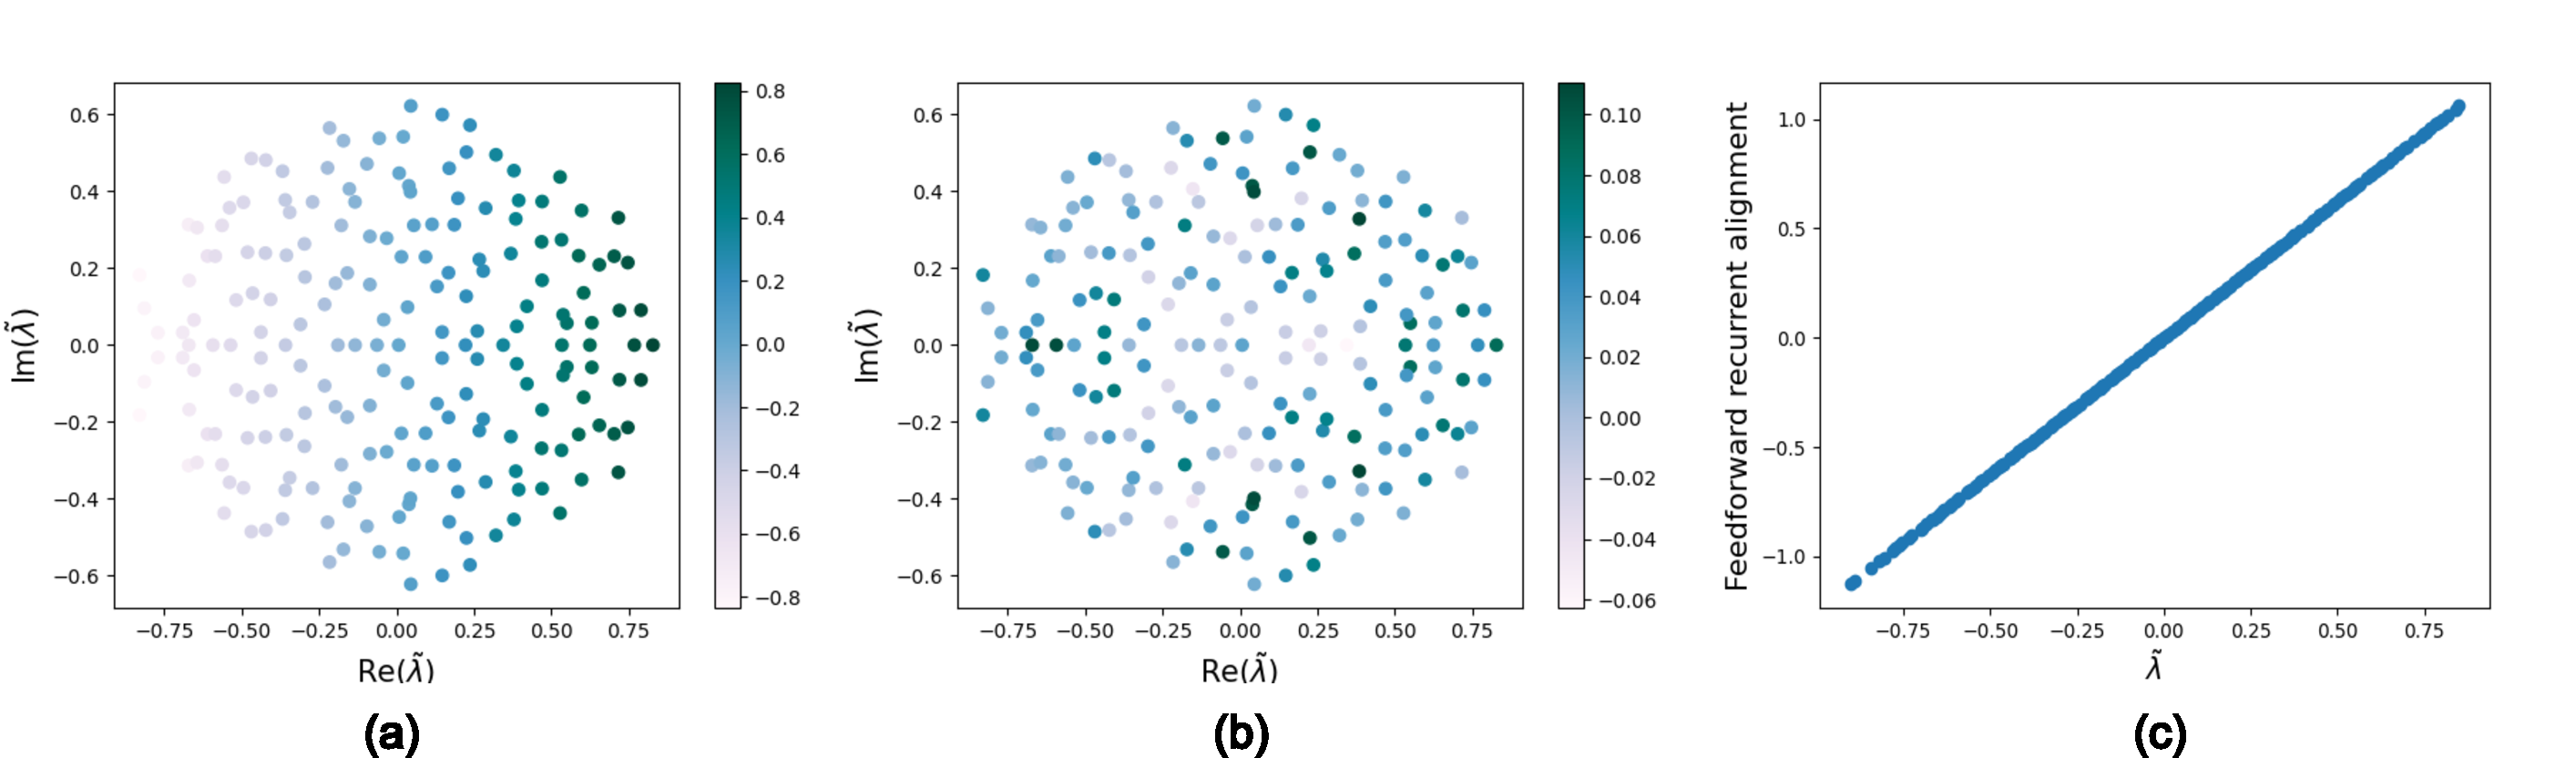
\includegraphics[width=\textwidth]{../figures/ffrec_eigval_proportion.pdf}
%			\caption{text}
%		\end{figure}
		\begin{figure}[H]
			\centering
			\begin{subfigure}[b]{0.425\textwidth}
				\includegraphics[width=\textwidth]{../figures/ffrec_eigval_real_part(2).pdf}
				\caption{}
				\label{fig:ffrec_real_part}
			\end{subfigure}
			\hfill
			\begin{subfigure}[b]{0.425\textwidth}
				\includegraphics[width=\textwidth]{../figures/ffrec_eigval_mag(2).pdf}
				\caption{}
				\label{fig:ffrec_mag}
			\end{subfigure}
%			\begin{subfigure}[b]{0.3\textwidth}
%				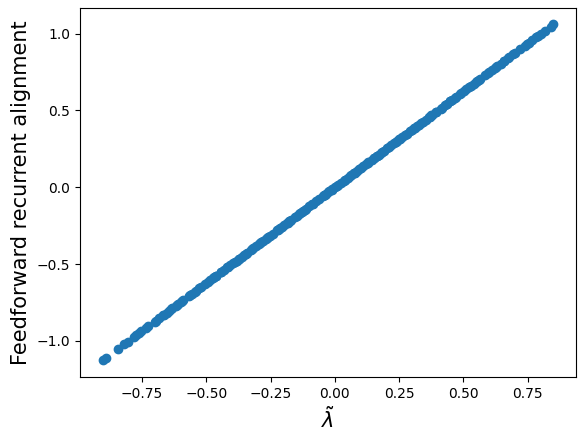
\includegraphics[width=\textwidth]{../figures/ffrec_eigval_symmetrized_J.png}
%				\caption{}
%			\end{subfigure}
			\caption[Correlation between eigenvalues and feedforward recurrent alignment of modifications for full-rank asymmetric RNNs]{\textbf{Correlation between eigenvalues and feedforward recurrent alignment of modifications for full-rank asymmetric RNNs.} To verify the considered modifications from section \ref{sec:modify_ffrec_alignment_score}, a monotonously positive correlation between eigenvalues and feedforward recurrent alignment is necessary. Represent the correlation in the complex plane, since eigenvalues are complex. The color-bar indicates the score of feedforward recurrent alignment. The darker the color, the larger the alignment score.  \textbf{(a)} Representation of alignment score calculated with modification \ref{sec:modicication_real_part} by eq.(\ref{eq:ffrec_real_part}) in complex plane. \textbf{(b)} Representation of alignment score calculated with modification \ref{sec:modification_magnitude} by eq.(\ref{eq:ffrec_mag}) in complex plane.}
		\end{figure}
	
	% Conclusion and mathematical explanation of Results for the proportionality.
	\vspace{0.5cm}
	\paragraph{Modification 1}: Apply the real part of complex inputs with eq.(\ref{eq:ffrec_real_part}).
	
	With the feedforward recurrent alignment, we mainly consider the correlation between alignment score and corresponding eigenvalues. Inserting inputs $h$ aligned to eigenvectors, for simplicity $h := e_i \in \mathbb{C}^{n \times 1}$ into eq.(\ref{eq:ffrec_real_part}), it leads to
		\begin{equation}
			\nu_{\text{Re}} = \frac{\text{Re}(e_i)^T J \text{Re}(e_i)}{\Vert \text{Re}(e_i)\Vert^2} \, .
		\end{equation}
	Because $\Vert e_i \Vert = c \Vert \text{Re}(e_i) \Vert$ with $c \in \mathbb{R_{+}}$ a general positive constant, we could get the proportionality between alignment score $\nu_{\text{Re}}$ and the real part of eigenvalues $\text{Re}(\lambda_i)$ of $J$ :
		\begin{equation}
			\begin{split}
				\nu_{\text{Re}} & = c \text{Re}\left( \frac{e_i}{\Vert e_i \Vert} \right)^T J \, \text{Re}\left( \frac{e_i}{\Vert e_i \Vert} \right) \\
				& = c \text{Re} \left( \frac{e_i^T}{\Vert e_i \Vert} J \frac{e_i}{\Vert e_i \Vert} \right) \\
				& = c \text{Re}(\lambda_i) \, ,
			\end{split}
		\end{equation}
	with $c$ a general positive constant.
	
	The positive correlation between alignment and the real part of eigenvalues $\lambda_i$ could also be observed in representation in the complex plane (Figure \ref{fig:ffrec_real_part}). With increasing the real part of the eigenvalue, the size of the alignment score also becomes larger. 
	%Therefore, the increase of the feedforward recurrent alignment score can be captured by an increase in the real part of eigenvalues.
	A better alignment between inputs and a certain dominant activity pattern is thus the only reason for the increase in the feedforward recurrent alignment score. Since the alignment score only depends on the real part, there is no correlation found in the direction of the imaginary part of eigenvalues. 
	\vspace{1cm}
	\paragraph{Modification 2}: Apply the magnitude for each neuron input eq.(\ref{eq:ffrec_mag}).
	
	When the inputs are aligned to eigenvectors $e$ of interaction matrix $J$, the feedforward recurrent alignment could be modified with $\vert e \vert := (\vert e_{i} \vert)_{i = 1, ..., n} \in \mathbb{R}^{n \times 1}$. Since the euclidean norm of vector $\vert e \vert$ is the same as the norm directly on the complex eigenvector $\Vert e \Vert_2$, the final feedforward recurrent alignment score from eq.(\ref{eq:ffrec_mag}) can be formulated as following:
		\begin{equation}
			\begin{split}
				\nu_{\text{mag}} & = \frac{\vert e \vert^T J \vert e \vert}{\Vert e \Vert^2} \\
			%	& = \frac{\sum_{j=1}^{n} \sqrt{x_j^2 + y_j^2} \left( \sum_{i = 1}^{n} \sqrt{x_i^2 + y_i^2} J_ij \right)}{\sum_{i=1}^{n}}
				& = \frac{\sum_{j=1}^{n} \vert e_{j} \vert \left( \sum_{i = 1}^{n} \vert e_{i} \vert J_{ij} \right)}{\Vert e \Vert^2} \, ,
			\end{split}
		\end{equation}
	where $e_i, e_j$ are the $i$-th and $j$-th element of the vector $e$, and $J_{ij}$ the matrix element at $i$-th row and $j$-th column. 
	
	No direct proportionality between the alignment score and corresponding eigenvalues $\lambda$ can be established. The lack of correlation is also represented in the complex plane (Figure \ref{fig:ffrec_mag}). 
	\vspace{1cm}
	\paragraph{Modification 3}: Align the inputs to eigenvectors of symmetrized network eq.(\ref{eq:ffrec_symmetrized}).
	
	Instead of aligning the inputs to eigenvectors of original asymmetric RNNs and thinking about modifications of complex eigenvectors to calculate the feedforward recurrent alignment score, we now align the inputs to real eigenvectors $\tilde{e}$ from symmetrized interaction matrix $\tilde{J}$ as an approximation. However, the alignment score is still being projected to the original asymmetric RNNs defined in eq.(\ref{eq:ffrec_symmetrized}). 
	Despite of original asymmetric interaction matrix for the feedforward recurrent alignment score, there is still a proportionality between the eigenvalues of the symmetrized network and alignment score, shown in Figure \ref{fig:ffrec_symmetrized}. 
	
	The kept proportionality can also be obtained analytically. With the formulation of symmetrized interaction matrix through eq.(\ref{eq:symmetrized_J}), it follows with the help of definition for $\nu_{\text{sym}}$ from eq.(\ref{eq:ffrec_symmetrized}),
	
		\begin{equation}
			\begin{split}
				&\frac{\tilde{e}^T \tilde{J} \tilde{e}}{\Vert \tilde{e} \Vert^2} = \frac{\tilde{e}^T \frac{J + J^T}{2} \tilde{e}}{\Vert \tilde{e} \Vert^2} = \frac{1}{2} \left( \frac{\tilde{e}^T J \tilde{e}}{\Vert \tilde{e} \Vert^2} + \frac{\tilde{e}^T J^T \tilde{e}}{\Vert \tilde{e} \Vert^2} \right) \\
				\Rightarrow \,  & 2 \frac{\tilde{e}^T \tilde{J} \tilde{e}}{\Vert \tilde{e} \Vert^2} - \frac{\tilde{e}^T J^T \tilde{e}}{\Vert \tilde{e} \Vert^2} = \frac{\tilde{e}^T J \tilde{e}}{\Vert \tilde{e} \Vert^2} \\ 
				\Rightarrow \, & 2 \tilde{\lambda} - c = \frac{\tilde{e}^T J \tilde{e}}{\Vert \tilde{e} \Vert^2} \text{ with } c := \frac{\tilde{e}^T J^T \tilde{e}}{\Vert \tilde{e} \Vert^2} \in \mathbb{R} \text{ and $\tilde{\lambda}$ the corresponding eigenvalue of $\tilde{e}$} \\
				\Rightarrow \, & \nu_{\text{sym}} = \frac{\tilde{e}^T J \tilde{e}}{\Vert \tilde{e} \Vert^2} \propto \tilde{\lambda} \, .
			\end{split}
		\end{equation}
	\begin{SCfigure}[0.95][h]
		\centering
		\caption[Positive correlation between feedforward recurrent alignment score and eigenvalues of symmetrized network as modification for asymmetric RNNs]{\textbf{Positive correlation between feedforward recurrent alignment score and eigenvalues of symmetrized network as modification for asymmetric RNNs.} Align the inputs to the eigenvectors of the symmetrized network while keeping feedforward recurrent alignment obtained by the original asymmetric interaction matrix with eq.(\ref{eq:ffrec_symmetrized}). The correlation between the alignment score (y-axis) to the corresponding eigenvalues of the symmetrized network (x-axis) remains positive.}
		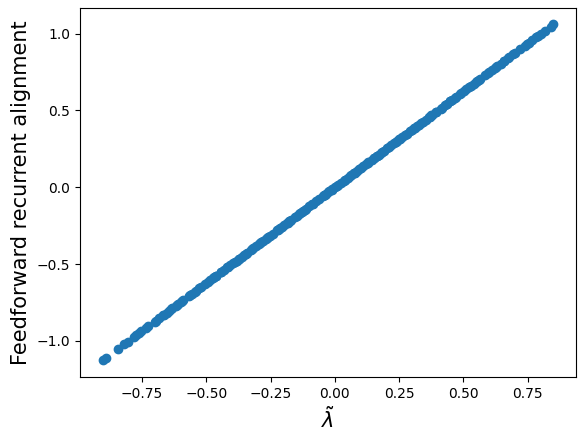
\includegraphics[width=0.48\textwidth]{../figures/ffrec_eigval_symmetrized_J.pdf}
		\label{fig:ffrec_symmetrized}
	\end{SCfigure}
	%\vspace{0.3cm}
	\paragraph{Section conclusion} After the analysis above for all modifications, our expectation of a contained positive correlation is kept when considering the real part (modification 1) and alignment with the symmetrized interaction matrix (modification 3). The variant with magnitude (modification 2) fails to fulfill the expected correlation. Thus, we will leave modification 2 out without further analysis of response properties in the following section. 
	
	\subsubsection{Verifying Response Properties with modified Feedforward Recurrent Alignment} \label{sec:asym_ffrec_response}
	
	After verifying the expected correlation between the feedforward recurrent alignment score and eigenvalues, we next test if the remaining two modifications could still reflect the four experimental observations listed at the beginning of the section \ref{sec:asymmetric_results}. 
	
	For this, we align the inputs to eigenvectors of the asymmetric recurrent network to compute the four response properties and compare them with experimental observations from \cite{tragenap2023nature}. The following modifications for the modeling are taken into account:
	\begin{itemize}
		\item modification 1: consider only the real part of eigenvectors eq.(\ref{eq:ffrec_real_part}). 
		\item modification 3: align the inputs to eigenvectors of the symmetrized interaction matrix but calculates the alignment score still with the original asymmetric network eq.(\ref{eq:ffrec_symmetrized}). 
	\end{itemize}
	
	For the modeling, the asymmetric RNNs are constructed with a certain degree of symmetry with eq.(\ref{eq:asym_interaction_matrix}). We therefore also controlled how much the degree of symmetry influences the results. 
	
	%\vspace{0.3cm}
	\paragraph{Trial-to-trial Correlation}
	
	Trial-to-trial correlation is the averaged correlations between single trial responses defined by eq.(\ref{eq:ttc_sym}). From the experimental results in \cite{tragenap2023nature}, a positive correlation between feedforward recurrent alignment and trial-to-trial correlation is expected. Under various degree of symmetry, the positive correlation should still be kept.
	
		\begin{figure}[H]
			\centering
			\includegraphics[width = \textwidth]{../figures/ttc_asym(2).pdf}
			\caption[Trial-to-trial correlation concerning feedforward alignment and degree of symmetry in full-rank asymmetric RNNs]{\textbf{Trial-to-trial correlation concerning feedforward alignment and degree of symmetry in full-rank asymmetric RNNs.} Color-coded is the degree of symmetry $a$ (see legend). The green dots with $a=1.0$ illustrate the case of symmetric RNNs. The darkest purple dots $a=0.0$ represent the asymmetric network without any degree of symmetry. The x-axis shows the alignment score calculated with considered modifications 1 and 3, and the y-axis indicates the trial-to-trial correlation calculated with aligned inputs through eq.(\ref{eq:ttc_sym}) \textbf{Left}: Results generated with modification 1 (only consider real part). \textbf{Right}: Result with modification 3 (symmetrized interaction matrix).}
			\label{fig:ttc_asym}
		\end{figure}
	
	The results in Figure \ref{fig:ttc_asym} show that the trend of positive correlation between trial-to-trial correlation and feedforward recurrent alignment score keeps while the network increases its asymmetry for both modifications 1 and 3. 
	
	However, when the network is fully asymmetric, the correlation has a larger dispersion with modification 1. We suspect that the reason is that in the case of full asymmetry, more information got lost if only considering information from the real part of the aligned inputs. 
	
	If there is a certain degree of symmetry, a part of the information originates from the symmetric structure. For this part, no information gets lost when only taking the real part of aligned inputs. On the other hand, aligning to fully asymmetric RNNs ($a = 0.0$ in Figure \ref{fig:its_asym} left panel) and only taking the real part of aligned inputs, all neurons receive then incomplete information. Therefore, the correlation between evoked patterns will be disturbed mostly. 
	
	In the case of modification 3, the correlation is almost maintained the overall degree of symmetry as expected, shown in Figure \ref{fig:its_asym} right panel. 
	
	%\vspace{0.3cm}
	\paragraph{Intra-trial Stability}
	
	Intra-trial stability is the averaged time-delayed activity correlation inside one single trial quantified by eq.(\ref{eq:its_sym}). As the name indicates, it shows how stable the information is represented inside one trial. According to the result from symmetric RNNs (Figure \ref{fig:its_ffrec_sym}), we expect a similar exponential positive correlation also with full-rank asymmetric RNNs. The degree of symmetry should also not influence the result significantly under the assumption that the hypothesis works well with asymmetric RNNs generally.
	
		\begin{figure}[H]
			\centering
			\includegraphics[width=\textwidth]{../figures/its_asym(2).pdf}
			\caption[Intra-trial stability with respect to feedforward recurrent alignment and the influence from the degree of symmetry in full-rank asymmetric RNNs]{\textbf{Intra-trial stability with respect to feedforward recurrent alignment and the influence from the degree of symmetry in full-rank asymmetric RNNs.} For multiple degrees of symmetry $a$, different color dots are applied shown in the legend. From complete symmetric ($a = 1.0$ as the control group) to full asymmetric ($a = 0.0$) RNNs, the corresponding feedforward recurrent alignment (x-axis) is plotted against the intra-trial stability (y-axis). \textbf{Left}: Results with modification 1 (only real part of aligned inputs). \textbf{Right}: Results with modification 3 (align input to symmetrized network).}
			\label{fig:its_asym}
		\end{figure}
	
	%We suspect with a similar reason as in trial-to-trial correlation that for modification 1, the loss of imaginary part information of aligned inputs could lead to increased dispersion with the network becoming more asymmetric (Figure \ref{fig:its_asym} left panel). 
	In the left panel of Figure \ref{fig:its_asym}, the dispersion increased when the network become more symmetric. We suspect with a similar reason as in trial-to-trial correlation that for modification 1, which is the loss of imaginary part information of aligned inputs.
	
	For modification 3, the expected positive correlation between intra-trial stability and feedforward recurrent alignment score is kept. However, we also observe that the influence of the degree of symmetry influences here is more pronounced than in trial-to-trial correlation (Figure \ref{fig:ttc_asym} right panel). 
	It is perhaps because the intra-trial stability is more sensitive to the information lost than trial-to-trial correlation. With the increased asymmetry, more information got lost during symmetrization. Imagine if having a total symmetric network, the result of symmetrization is the network itself, and therefore no information is lost during the symmetrization. However, if having a fully asymmetric RNN, after symmetrization, complex eigenvectors are transformed into real-number eigenvectors. This could lead to the loss of information in those eigenvectors that characterize the asymmetric RNN.
	%information stored in complex eigenvectors gets transformed to lower dimension real eigenvectors. 
	Thus, when aligning inputs to the symmetrized interactions, transformed information could be the reason for the influence of the degree of symmetry. 
	
	%\vspace{0.5cm}
	\paragraph{Dimensionality}
	
	Dimensionality reflects the complexity of the information encoded by activity patterns. A high dimensional activity pattern needs more orthogonal activity patterns for representation than a low dimensional activity pattern and thus indicates larger variability and higher complexity of contained information \cite{tragenap2023nature, bartolo2020dimensionality, badre2021dimensionality}. We continuing for modeling the dimensionality with modifications 1 (consider real part) and 3 (symmetrization of asymmetric RNNs), which change the eigenvectors for the construction of input covariance and the eigenvalues for analytical calculation of effective dimensionality (section \ref{sec:modification_asym} eq.(\ref{eq:modifications_dim}), (\ref{eq:modification_eff_dim})). 
	If both modifications work well, the results should be similar to results from symmetric RNNs (Figure \ref{fig:dim_sym}b). 
	%A low degree of symmetry is allowed to lead to a small range of dispersion, which however should still keep the tendency of decreased dimensionality with increased feedforward recurrent alignment score. % Refer calculation in method + Expectiations
	
	% Reason for left: the analytical solution under assumption that the basis of Sigma_Dim are orthogonal-- got lost with Re(e). Therefore large difference between analytical and empirical solution. --> at this step the modification 1 is also not good. Could let out. 
	Different from the results in Figure \ref{fig:dim_sym}b, with modification 1 (Figure \ref{fig:dim_asym} left panel), the empirical dimensionality (eq.(\ref{eq:dim_empirical_sym})) differs a lot from the analytical calculation (eq.(\ref{eq:dim_analytical_sym})). Moreover, there is no significant correlation between dimensionality and feedforward recurrent alignment in the empirical modeling as long as asymmetric structure is included. There is a substantial mismatch between the analytical results and the empirical approximations. The reason for those phenomena could be the loss of orthogonality between the real part of eigenvectors, that is 
	\begin{equation}
		e_i \perp e_j  \, \, \nRightarrow \text{Re}(e_i) \perp \text{Re}(e_j) \, \, \forall i, j = 1, ..., n \, .
	\end{equation}
	As a result, the covariance matrix $\Sigma^{\text{Dim}}$ from eq.(\ref{eq:modifications_dim}) is not necessarily constructed with orthogonal vectors anymore, which contradicts the definition of covariance matrix. 
	%which contradicts the assumption of reflecting dimensionality by projecting activity pattern on orthogonal patterns that are also applied to construct covariance matrix. 
	
		\begin{figure}[H]
			\centering
			\includegraphics[width=\textwidth]{../figures/dim_asym(2).pdf}
			\caption[Analytical and empirical effective dimensionality with respect to the feedforward recurrent alignment score and the degree of symmetry in asymmetric RNNs]{\textbf{Analytical and empirical effective dimensionality with respect to the feedforward recurrent alignment score and the degree of symmetry in asymmetric RNNs.} The full symmetric recurrent network ($a = 1.0$) is a control for other cases. When $a = 0.0$, the RNN is fully asymmetric. The dots represent the empirical approximation for effective dimensionality eq.(\ref{eq:dim_empirical_sym}). The lines are for the analytical calculation for dimensionality adjusted to modification 1 and 3 (section \ref{sec:modification_asym} eq.(\ref{eq:modifications_dim}), (\ref{eq:modification_eff_dim})). \textbf{Left}: Results with modification 1 (only real part of aligned inputs and eigenvalues for analytical dimensionality). \textbf{Right}: Results with modification 3 (align inputs to symmetrized interaction matrix).}
			\label{fig:dim_asym}
		\end{figure}
	
	With modification 3, the results fulfill largely our expectations: the negative correlation between dimensionality and feedforward recurrent alignment is kept in both analytical and empirical approximations. Little dispersion could be due to the structural information lost during symmetrization. 
	
	Thus, until this step, we would also drop modification 1 and only further consider modification 3. 
	
	\paragraph{Alignment to spontaneous activity}
	The alignment of the evoked activity pattern to the endogenous pattern measures the overlap between their variance ratio curves explained by principal components of endogenous pattern eq.(\ref{eq:var_explain_spont_act_sym}). For example the overlaps between curves in Figure \ref{fig:variance_ratio_sym}. Only modification 3 is now left for the evaluation. 
	
	Similar to prior cases, if the modification works, we expect the correlation between alignment to spontaneous activity and feedforward recurrent alignment score to be similar to symmetric RNNs in Figure \ref{fig:align_spont_sym}. The alignment to spontaneous activity is modified with eq.(\ref{eq:Sigma_spont_asym}) and calculated with eq.(\ref{eq:align_to_spont_act_sym}). 
	
	As shown in Figure \ref{fig:align_to_spont_asym}, the dispersion increases with the degree of asymmetry due to the increased information lost. But the general tendency that the alignment of evoked activity pattern to spontaneous activity becomes larger when the inputs are aligned to more dominant eigenvectors of symmetrized interaction matrix is conserved. With a high degree of symmetry, for example, $a = 0.75$, the correlation is very similar to it with total symmetric recurrent network.
	
	\begin{SCfigure}[0.9][h] 
		\centering
		\caption[Alignment to spontaneous activity with respect to the feedforward recurrent alignment and influence from the degree of symmetry  for asymmetric RNNs with symmetrized interactions]{\textbf{Alignment to spontaneous activity with respect to the feedforward recurrent alignment and influence from the degree of symmetry  for asymmetric RNNs with symmetrized interactions.} As a control group,a fully symmetric RNN ($a=1.0$) is represented with dark green dots. For different degrees of symmetry from $a = 0.75$ to $0$, the darker the dots' color, the more asymmetry is in the network. Only modification 3 is evaluated for alignment to spontaneous activity.}
		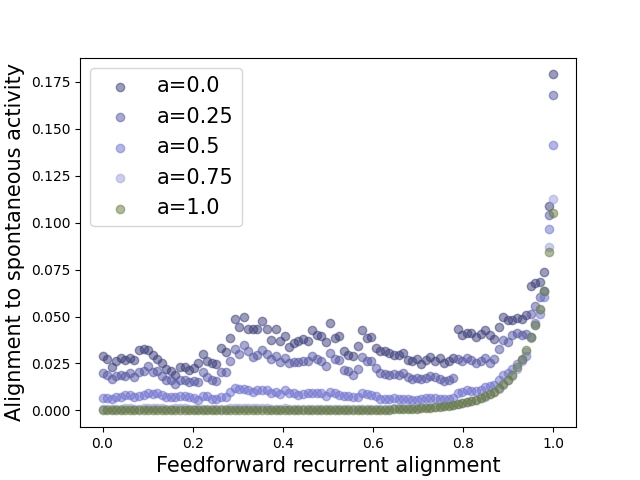
\includegraphics[width=0.5\textwidth]{../figures/align_to_spont_asym_symmetrized_rescaled.pdf}
		\label{fig:align_to_spont_asym}
	\end{SCfigure}

	\vspace{0.5cm}
	\paragraph{Section conclusion}
	After evaluating the rest of modifications 1 (consider real part of complex eigenvectors) and 3 (symmetrization of asymmetric RNNs) with four perspectives of response properties, modification 1 is filtered out because of the lack of orthogonality between eigenvectors after modification. This could be the reason for the large inconsistency between analytical and empirical approximations of effective dimensionality.
	
	Modification 3 performs at the end the best through all four response properties, and could generally fulfill the expectations of correlations between the response properties and feedforward recurrent alignment. 
	
	Therefore, modification 3 which aligns the inputs to asymmetric RNNs with a symmetrized interaction matrix is considered to be a good candidate for modeling feedforward recurrent alignment hypothesis in asymmetric recurrent networks.
	
	\clearpage
	\subsection{Modeling Feedforward Recurrent Alignment Hypothesis on Low-rank Recurrent Neural Networks (Low-rank RNNs)} \label{sec:low_rank_result}
	Although fully recurrent connectivity structure is one of the most popular network models for theoretical neuroscience, there are experimental recordings suggesting that the transformation of sensory stimuli into motor outputs relies on low-dimensional dynamics at the population level \cite{mastrogiuseppe2018linking}. Therefore, the low-rank connectivity structure can be a good candidate for understanding the neural mechanism from another perspective. 
	
	We hence also try to model the feedforward recurrent alignment hypothesis on the low-rank RNNs to discover if the hypothesis modeling adapted from full-rank RNNs also could work with low-rank RNNs. 
	% The logic line of the discovery. Which structure does the section follow.
	Hereby, we consider both symmetric and asymmetric RNNs with constructions with and without noise described in section \ref{sec:low_rank_construct} by eq.(\ref{eq:low_rank_RNN_without_noise}) and eq.(\ref{eq:low_rank_with_noise}). Under symmetric or asymmetric conditions, we go through both constructions with the four response properties in correlation with the feedforward recurrent alignment score as for full-rank RNNs before. Those four response properties are trial-to-trial correlation, intra-trial stability, dimensionality, and alignment to spontaneous activity. %The method will be dropped out here if the expectations are not fulfilled and the rest of results are contained in the Appendix. %TODO: Appendix write and link here. 
	
	\subsubsection{Evaluation of Feedforward Recurrent Alignment in symmetric Low-rank RNNs based on response properties}
	We first consider symmetric low-rank networks in constructions with and without noise. For each case, the results of response property analysis based on the modeling of the feedforward recurrent alignment hypothesis for symmetric networks are evaluated with correlations between them. 
	
	\paragraph{Low-rank RNNs without random noise}
	% Eigenvalue distribution (figure, rank = 1, n = 200) --> only one eigenvalue = 0.85, rest = 0 + explain (update 05.12.)
	The formulation of low-rank RNNs is followed by eq.\ref{eq:sym_low_rank} with the rank $G$ significantly smaller than the number of neurons $n$. The eigenvalues of symmetric low-rank RNNs are real numbers. 
		\begin{SCfigure}[0.9][h] 
			\centering 
			\caption[Eigenvalue distribution of symmetric low-rank RNNs without random noise]{\textbf{Eigenvalue distribution of symmetric low-rank RNNs without random noise.} The eigenvalues of symmetric low-rank RNNs are real numbers (x-axis). With rank $G = 1 \ll n = 200$ the number of neurons, $1$ eigenvalue takes the value of normalization factor $R = 0.85$, and the rest $n-G = 199$ eigenvalues equal $0$. }
			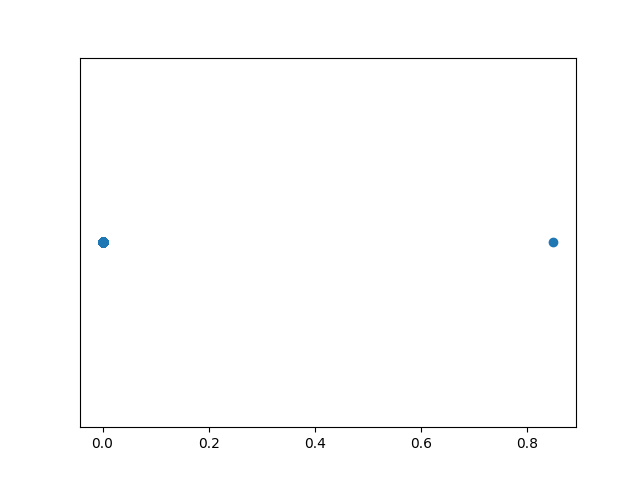
\includegraphics[width=0.5\textwidth]{../figures/eigval_low_rank_sym_no_noise.png}
			\label{fig:eigval_low_rank_without_noise}
		\end{SCfigure}
	
	As shown in Figure \ref{fig:eigval_low_rank_without_noise}, only two real eigenvalues are seen. A number of $G$ eigenvalues equal the normalization factor $R < 1$ that limits the value range by eq.(\ref{eq:eigval_normal}). The rest of $n-G$ eigenvalues take the value $0$. 
	
	The phenomenon of bi-polarized eigenvalue distribution is due to the construction of low-rank RNNs here. If considering the case of having the left connectivity vectors as orthonormal basis for construction of RNNs from eq.(\ref{eq:sym_low_rank}), which is
		\begin{equation} \label{eq:sym_low_rank_eigval}
			J = \frac{1}{n}\sum_{g =1}^{G} l^{(g)} l^{(g)T} = \sum_{g =1}^{G} \frac{1}{n} l^{(g)} l^{(g)T}\, . 
		\end{equation}
	If the rank equals the number of neurons, $G = n$, the formulation of low-rank matrix eq.(\ref{eq:sym_low_rank_eigval}) is at the same time a symmetric full rank matrix with eigenvectors $\left\{l^{(g)}\right\}$ and all eigenvectors correspond to the same eigenvalue $\frac{1}{n}$. Since the eigenvalues are re-scaled by parameter $R < 1$ to enable the stable steady state, the eigenvalues are equal to $R$ based on eq.(\ref{eq:eigval_normal}). 
	
	Now, if the rank $G$ is smaller than the number of neurons $n$, the formulation of low-rank RNN eq.(\ref{eq:sym_low_rank_eigval}) can be rewritten as 
		\begin{equation} \label{eq:sym_low_rank_without_noise_eigval}
			J = \sum_{g =1}^{G} \frac{1}{n} l^{(g)} l^{(g)T} + 0 = \sum_{g =1}^{G} \frac{1}{n} l^{(g)} l^{(g)T} + \sum_{g =G}^{n-G} 0 l^{(g)} l^{(g)T} \, .
		\end{equation}
	So, there are $G$ basis vectors that have eigenvalue $\frac{1}{n}$, which is further re-scaled to $R < 1$. The rest of $n-G$ eigenvectors have eigenvalue $0$. This then results the eigenvalue distribution shown in Figure \ref{fig:eigval_low_rank_without_noise}. 
	
	We first look at the trial-to-trial correlation and expect a positive correlation with the feedforward recurrent alignment. When aligning the inputs to the symmetric recurrent alignment, the inputs-distribution has the mean vector matched to the eigenvectors of the low-rank interaction matrix $J$. Due to the feedforward recurrent alignment formulation, the alignment scores are equal to the corresponding eigenvalues because of eq.(\ref{eq:ffrec_equals_eigval}). 
	
	Since there are only two eigenvalues $R$ and $0$ for the rank $G$ smaller than number of neurons $n$, we assume that there is no continuous correlation but two groups of trial-to-trial correlation values. However, low feedforward recurrent alignment should still correlate with a small trial-to-trial correlation value and a large alignment score with a big trial-to-trial correlation. We expect therefore here a discontinuous positive correlation between trial-to-trial correlation and feedforward recurrent alignment. 
%		\begin{SCfigure}[0.9][h]
%			\centering
%			\caption{\textbf{Trial-to-trial correlation against the feedforward recurrent alignment for low-rank symmetric RNNs without noise.} The positive correlation between feedforward recurrent alignment and trial-to-trial correlation is discontinuous due to the number of eigenvalues under low rank. If having rank $G = 1$, only one feedforward recurrent alignment score take the values $R = 0.85$. The rest concentrates at alignment score $0$ with low trial-to-trial correlation. }
%			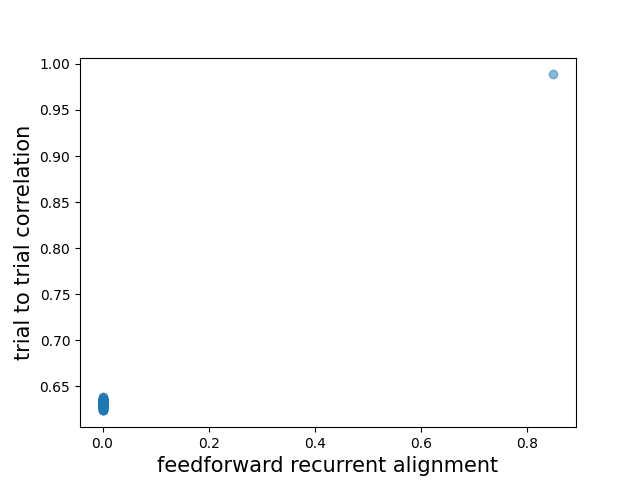
\includegraphics[width=0.5\textwidth]{../figures/low_rank_sym_ttc.png}
%			\label{fig:ttc_low_rank_sym_no_noise}
%		\end{SCfigure}
	
	As the result in Figure \ref{fig:ttc_its_low_rank_sym_no_noise}a shows, the trial-to-trial correlation distributes separately into two groups due to the distribution of eigenvalues. Also as expected, there is still a positive correlation between feedforward recurrent alignment score and trial-to-trial correlation.
	%a small feedforward recurrent alignment score corresponds with small a trial-to-trial correlation and a large feedforward recurrent alignment with a large trial-to-trial correlation.
	%When the feedforward recurrent alignment is low, the trial-to-trial correlation concentrates also at the small number range. The trial-to-trial correlation increases when the feedforward recurrent alignment takes the larger eigenvalue. 
	
%		\begin{SCfigure}[0.9][h]
%			\centering
%			\caption{text}
%			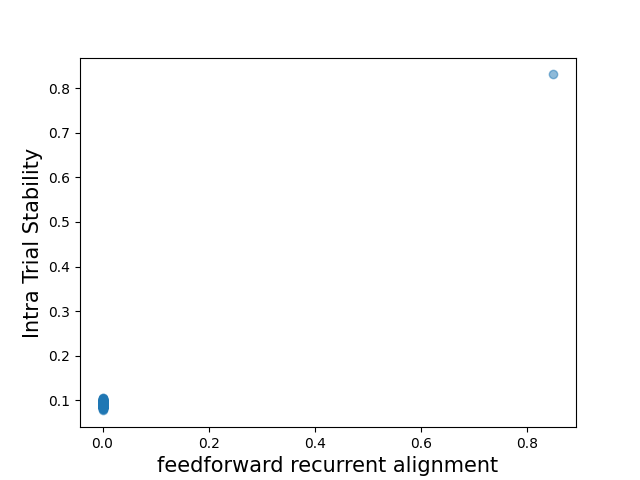
\includegraphics[width=0.5\textwidth]{../figures/its_low_rank_sym_without_noise.png}
%		\end{SCfigure}
%	
		\begin{figure}[H]
			\centering
			\begin{subfigure}[b]{0.45\textwidth}
				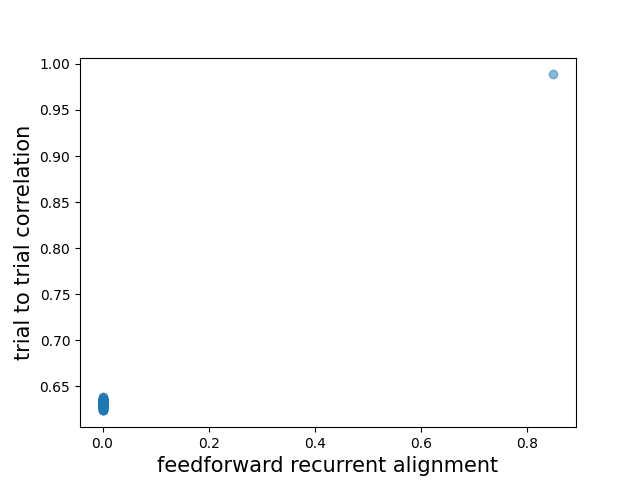
\includegraphics[width=\textwidth]{../figures/low_rank_sym_ttc.png}
				\caption{}
			\end{subfigure}
			\hfill
			\begin{subfigure}[b]{0.45\textwidth}
				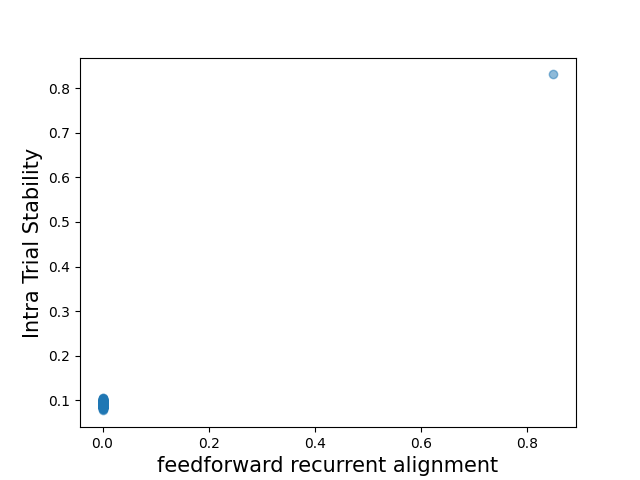
\includegraphics[width=\textwidth]{../figures/its_low_rank_sym_without_noise.png}
				\caption{}
			\end{subfigure}
			\newline
			\begin{subfigure}[b]{0.45\textwidth}
				\includegraphics[width=\textwidth]{../figures/dim_low_rank_sym_without_noise.png}
				\caption{}
			\end{subfigure}
			\hfill
			\begin{subfigure}[b]{0.45\textwidth}
				\includegraphics[width=\textwidth]{../figures/align_to_spont_low_rank_without_noise.png}
				\caption{}
			\end{subfigure}
			\caption[Correlation between response properties and feedforward recurrent alignment considering symmetric low-rank RNNs without random noise]{\textbf{Correlation between response properties and feedforward recurrent alignment considering symmetric low-rank RNNs without random noise.} Construct symmetric low-rank RNNs under the assumption of having left connectivity vectors equal to right connectivity vectors eq.(\ref{eq:sym_low_rank_eigval}). Rank $G$ is the number of connectivity vectors and is significantly smaller than the number of neurons $n$. Here $G = 1$ and $n = 200$. To evaluate the feedforward recurrent alignment hypothesis, the correlations between response properties and the modeled feedforward recurrent alignment score are considered. \\
			\textbf{(a)} Trial-to-trial correlation (y-axis) in correlation with feedforward recurrent alignment score (x-axis).\\
			\textbf{(b)} Intra-trial stability (y-axis) in correlation with feedforward recurrent alignment score (x-axis).\\
			\textbf{(c)} Dimensionality (y-axis) calculated analytically (green dots, eq.(\ref{eq:dim_analytical_sym})) and empirically (blue dots, eq.(\ref{eq:dim_empirical_sym})) in relationship with feedforward recurrent alignment score (x-axis).\\
			\textbf{(d)} Correlation between alignment to spontaneous activity (y-axis) and feedforward recurrent alignment score (x-axis).}
		
%			\caption{\textbf{Trial-to-trial correlation and intra-trial stability in correlation with feedforward recurrent alignment score for low-rank symmetric RNNs.} \textbf{(a)} Trial-to-trial correlation in relationship with feedforward recurrent alignment. \textbf{(b)} Intra-trial stability in relationship with feedforward recurrent alignment.\\ The positive correlation between feedforward recurrent alignment and trial-to-trial correlation \textbf{(a)} or intra-trial stability \textbf{(b)} is discontinuous due to the number of eigenvalues under low rank. If having rank $G = 1$, only one feedforward recurrent alignment score take the value $R = 0.85$, correlating with large trial-to-trial correlation \textbf{(a)} or intra-trial stability \textbf{(b)}. The rest concentrates at alignment score $0$ with low trial-to-trial correlation \textbf{(a)} or low intra-trial stability \textbf{(b)}. }
			\label{fig:ttc_its_low_rank_sym_no_noise}
		\end{figure}
	
	%TODO: Now also consider the other respose properties. 
	% its + reason for not going on with this approach
	Analogous to the trial-to-trial correlation, we receive the results for intra-trial stability (Figure \ref{fig:ttc_its_low_rank_sym_no_noise}b) and alignment to spontaneous activity (Figure \ref{fig:ttc_its_low_rank_sym_no_noise}c) also be a discontinuous positive correlation to feedforward recurrent alignment, meanwhile a discontinuous negative correlation for dimensionality (Figure \ref{fig:ttc_its_low_rank_sym_no_noise}d). Due to the same reason of existing only two groups of eigenvalues at $R$ and $0$, the intra-trial stability value, alignment to spontaneous activity, and dimensionality distribute also separately into two groups while keeping the expected correlations with feedforward recurrent alignment.
	
%	 Although the positive correlation of feedforward recurrent alignment with both trial-to-trial correlation and intra-trial stability is kept. Since the simple distribution of eigenvalues leads to trivial dynamics between response properties and feedforward recurrent alignment as well as some unwanted effects in dimensionality (Appendix), %TODO:linking
%	 we would rather abandon the formulation of low-rank RNNs for trying modeling feedforward recurrent alignment hypothesis. 
	
	\paragraph{Low-rank RNNs with random noise}
		%The same evaluations considering the response properties are also undertaken for the case when considering the random noise to symmetric low-rank RNNs. 
		\begin{figure}[H]
			\centering
			\begin{subfigure}[b]{0.45\textwidth}
				\centering
				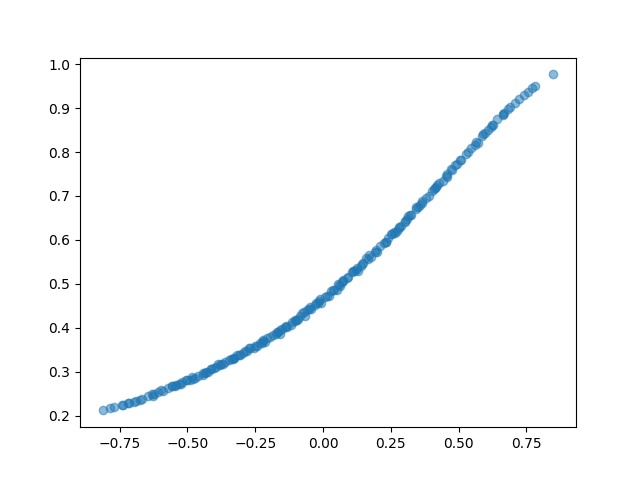
\includegraphics[width=\textwidth]{../figures/ttc_low_rank_sym_with_noise.png}
				\caption{}
			\end{subfigure}
			\hfill
			\begin{subfigure}[b]{0.45\textwidth}
				\centering
				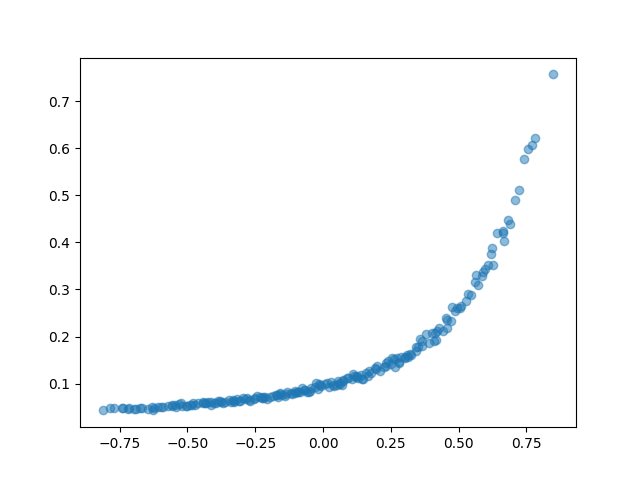
\includegraphics[width=\textwidth]{../figures/its_low_rank_sym_with_noise.png}
				\caption{}
			\end{subfigure}
			\newline
			\begin{subfigure}[b]{0.45\textwidth}
				\centering
				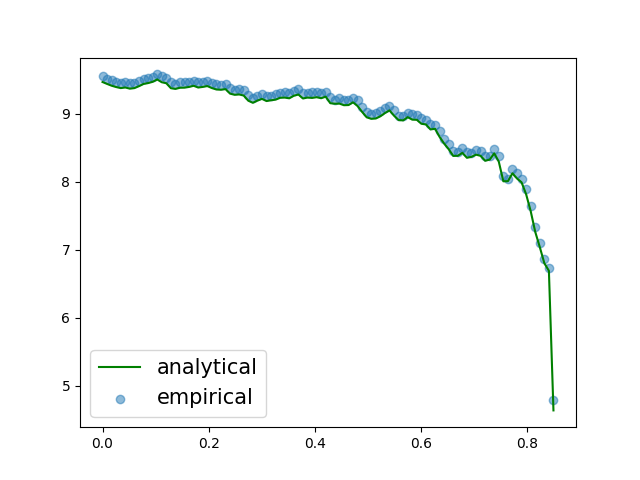
\includegraphics[width=\textwidth]{../figures/dim_low_rank_sym_with_noise.png}
				\caption{}
			\end{subfigure}
			\hfill
			\begin{subfigure}[b]{0.45\textwidth}
				\centering
				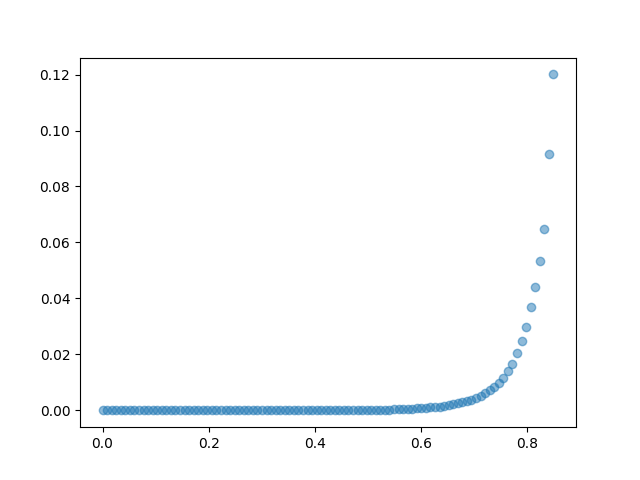
\includegraphics[width=\textwidth]{../figures/spont_align_low_rank_sym_with_noise.png}
				\caption{}
			\end{subfigure}
		\caption[Correlation between response properties and feedforward recurrent alignment in symmetric low-rank RNNs with random noise]{\textbf{Correlation between response properties and feedforward recurrent alignment in symmetric low-rank RNNs with random noise.} Besides the part of a low-rank matrix with rank $G$, low-rank RNNs with noise include an extra part of symmetrized random Gaussian matrix from eq.(\ref{eq:low_rank_sym_with_noise}). $G=1$ here.\\
		\textbf{(a)} Trial-to-trial correlation (y-axis) against feedforward recurrent alignmnet score (x-axis).\\
		\textbf{(b)} Intra-trial stability (y-axis) against feedforward recurrent alignment score (x-axis). \\
		\textbf{(c)} Dimensionality (y-axis) in dependence of feedforward recurrent alignment score (x-axis). Green dots represent the analytical calculation of dimensionality eq.(\ref{eq:dim_analytical_sym}) and blue dots for empirical approximation of eq.(\ref{eq:dim_empirical_sym})\\
		 \textbf{(d)} Alignment to spontaneous activity (y-axis) against feedforward recurrent alignment (x-axis).}
	 	\label{fig:result_sym_low_rank_with_noise}
		\end{figure}
%		\begin{figure}[H]
%			\centering
%			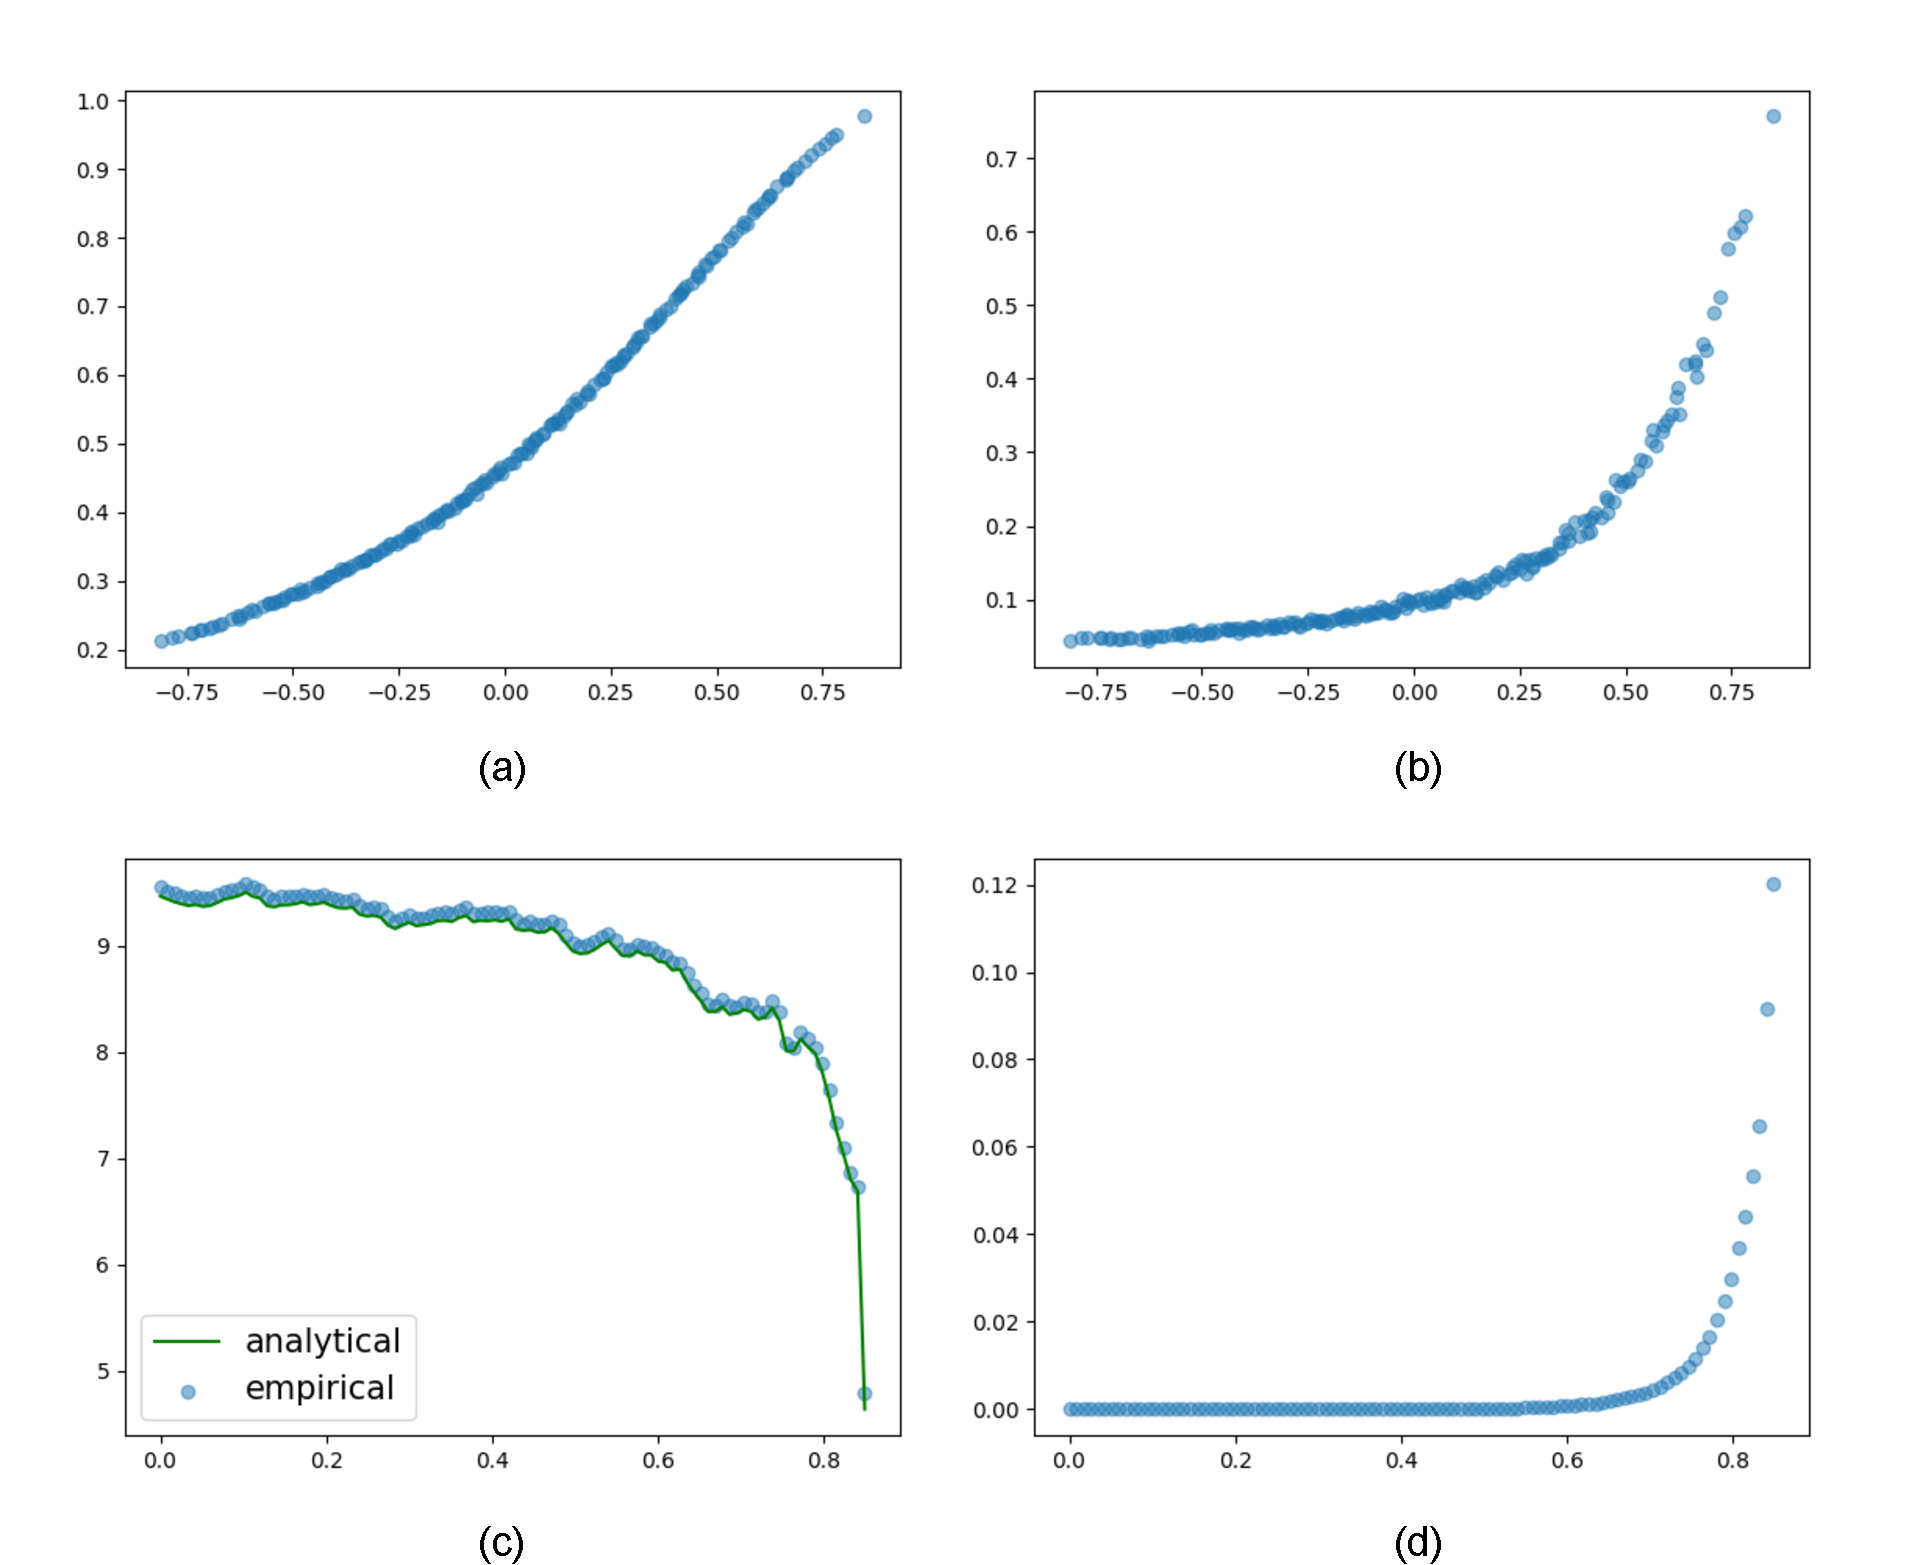
\includegraphics[width=0.8\textwidth]{../figures/low_rank_sym_with_noise.pdf}
%			\caption{\textbf{Correlation between response properties and feedforward recurrent alignment in low-rank RNNs with random noise.} Besides the part of a low-rank matrix with rank $G$, RNNs with noise includes an extra part of symmetrized random Gaussian matrix (\ref{eq:low_rank_sym_with_noise}). The rank of low rank part has the rank $G=1$.\\
%			\textbf{(a)} Trial-to-trial correlation (y-axis) against feedforward recurrent alignmnet score (x-axis). \textbf{(b)} Intra-trial stability (y-axis) against feedforward recurrent alignment score (x-axis). \textbf{(c)} Dimensionality (y-axis) in dependence of feedforward recurrent alignment score (x-axis). \textbf{(d)} Alignment to spontaneous activity (y-axis) against feedforward recurrent alignment (x-axis).}
%		\end{figure}
	
	Low-rank symmetric RNNs with random noise include an extra part of symmetrized Gaussian distributed matrix defined as  eq.(\ref{eq:low_rank_with_noise}) in section \ref{sec:ffrec_low_rank}. If analog to eq.(\ref{eq:sym_low_rank_eigval}) considering the right connectivity vectors equal to the left connectivity vectors, the symmetric low-rank RNNs with random noise can be formulated with a part of symmetric low-rank RNN and a part of symmetrized Gaussian distributed matrix $J_{\text{rand}}$. 
	\begin{equation} \label{eq:low_rank_sym_with_noise}
		J = \frac{1}{n}\sum_{g =1}^{G} l^{(g)} l^{(g)T} + J_{\text{rand}} \, .
	\end{equation}
	The symmetric random part $J_{\text{rand}}$ should provide more dynamics in the network. 
	
	Since $J_{\text{rand}}$ is a full-rank symmetric matrix, the final recurrent network $J$ is also a full-rank symmetric matrix despite the low-rank symmetric part with rank $G$. Therefore, the correlations between the response properties and feedforward recurrent alignment score are similar to the case of full-rank symmetric RNNs (Figure \ref{fig:ttc_ffrec_sym}, \ref{fig:its_ffrec_sym}, \ref{fig:dim_sym}, and \ref{fig:align_spont_sym}). 
	
	As a result, the feedforward recurrent alignment hypothesis can be modeled. The expected relationships between feedforward recurrent alignment and response properties from section \ref{sec:results_symmetric}) are fulfilled, as shown in Figure \ref{fig:result_sym_low_rank_with_noise}. However, the influence of low-rank construction is therefore overwritten by the random noise, which leads to the final dynamics not much different from the case with general random symmetric RNNs. 
	
	\paragraph{Section conclusion}
	
	Considering symmetric low-rank RNNs without random noise, the feedforward recurrent alignment keeps positive correlations to trial-to-trial correlation, intra-trial stability, and alignment to spontaneous activity. Besides, the expected negative correlation between dimensionality and feedforward recurrent alignment is also fulfilled. However, the network construction eq.(\ref{eq:sym_low_rank_eigval}) leads to a simple distribution of eigenvalues (Figure \ref{fig:eigval_low_rank_without_noise}) and in turn also the distribution of feedforward recurrent alignment score. As a result, only a simple discontinuous correlation of feedforward recurrent alignment to response properties can be observed (Figure \ref{fig:ttc_its_low_rank_sym_no_noise}). 
	
	If adding random noise to disturb the simple dynamics of symmetric low-rank RNNs with eq.(\ref{eq:sym_low_rank_eigval}), the final construction eq.(\ref{eq:low_rank_sym_with_noise}) is a full-rank symmetric RNN. As a result, the correlations of feedforawrd recurrent alignment to response properties are similar to the results observed in general symmetric RNNs from section \ref{sec:results_symmetric}. Although the expected phenomena are seen, the effect of low-rank RNNs cannot be significantly detected. 
	
	In total, after considering the symmetric low-rank RNNs with and without random noise, the feedforward recurrent alignment hypothesis can be modeled in both cases. The relationships between feedforward recurrent alignment and response properties also meet the expectations. %But either can have significant complex dynamics. Besides, the influence of the rank is also not observable. 
	
	\subsubsection{Different Constructions influence the impact of rank in Asymmetric Low-rank RNNs based on Response Properties}
	
	Asymmetric low-rank RNNs can have more complex dynamics than symmetric low-rank RNNs. Section \ref{sec:ffrec_low_rank} also introduces the construction of asymmetric low-rank RNNs with or without random noise. Generally, if taking the set of left connectivity vectors different from the set of right connectivity vectors, asymmetric matrices can be formulated by eq.(\ref{eq:low_rank_RNN_without_noise}), (\ref{eq:low_rank_with_noise}). 
	
	% Choose symmetrized method from privious results. 
	Since asymmetric low-rank RNNs are only a certain case of asymmetric RNNs with specific constructions, they also have the problem of complex eigenvectors and eigenvalues when modeling the feedforward recurrent alignment hypothesis. Therefore, from the previous results with general asymmetric RNNs, we choose modification 3 from section \ref{sec:modification_asym} with aligning inputs to symmetrized RNN because of the overall best performance among all considered modifications as mentioned in section \ref{sec:asymmetric_results}.

	\paragraph{Low-rank RNNs without random noise}
	
	Asymmetric low-rank RNNs without random noise consist of non-equal left and right connectivity vectors, which are mutually orthogonal illustrated in Figure \ref{fig:low_rank_RNN_without_noise}) and eq.(\ref{eq:low_rank_RNN_without_noise}). 
		\begin{figure}[H]
			\centering
			\begin{subfigure}[b]{0.3\textwidth}
				\centering
				\includegraphics[width=\textwidth]{../figures/eigval_distribution_asym_low_rank_without_noise.png}
				\caption{rank$=1$}
			\end{subfigure}
			\begin{subfigure}[b]{0.3\textwidth}
				\centering
				\includegraphics[width=\textwidth]{../figures/eigval_distribution_asym_low_rank_without_noise(2).png}
				\caption{rank$=5$}
			\end{subfigure}
			\begin{subfigure}[b]{0.3\textwidth}
				\centering
				\includegraphics[width=\textwidth]{../figures/eigval_distribution_asym_low_rank_without_noise(3).png}
				\caption{rank$=10$}
			\end{subfigure}
			\caption[Eigenvalue distribution in dependence of rank with asymmetric low-rank RNNs without random noise]{\textbf{Eigenvalue distribution in dependence of rank with asymmetric low-rank RNNs without random noise.} The asymmetric low-rank RNNs without random noise are constructed by mutually orthogonal non-equal left and right connectivity vectors defined by eq.(\ref{eq:low_rank_RNN_without_noise}). The number of vector pairs $G$ also determines the rank of the interaction matrix, which should be significantly smaller than the number of neurons $n$. The rank $G$ can influence the distribution of eigenvalues for asymmetric low-rank RNNs in complex plane. Plotting eigenvalues in the complex plane with x-axis for the real part and y-axis for the imaginary part. Low-rank RNNs with rank: \textbf{(a)} $G=1$. \textbf{(b)} $G=5$. \textbf{(c)} $G=10$. }
			\label{fig:eigval_distribution_asym_low_rank_without_noise}
		\end{figure}
	
	For symmetric low-rank RNNs without random noise, as long as the rank $G$ is significantly smaller than the number of neurons $n$ as defined, the distribution of eigenvalues is separated into two groups as in Figure \ref{fig:eigval_low_rank_without_noise} keeps unchanged independent of the rank. While for asymmetric low-rank RNNs without random noise, the influence of rank $G$ is more significant, as shown in Figure \ref{fig:eigval_distribution_asym_low_rank_without_noise}. 
	
	The construction of asymmetric low-rank RNNs without random noise defined by eq.(\ref{eq:low_rank_RNN_without_noise}) can be understood as $G$ pairs of presented connectivity vectors, while the rest of $n-G$ pairs are suppressed, rewritten with
		\begin{equation} \label{eq:asym_low_rank_RNNs_without_noise_eigval}
			J = \frac{1}{n} \sum_{g=1}^{G} l^{(g)} r^{(g)T} = \sum_{g=1}^{G} \frac{1}{n} l^{(g)} r^{(g)T} + \sum_{g=1}^{n-G} 0 l^{(g)} r^{(g)T} \, .
		\end{equation}
	Therefore, exactly $G$ number of eigenvalues do not concentrate at $0$ but the rest $n-G$ eigenvalues are. Since the mathematical construction eq.(\ref{eq:low_rank_RNN_without_noise}) for asymmetric low-rank RNNs is not an eigendecomposition, the eigenvalues after re-scaling by normalization parameter $R$ (method section \ref{sec:ffrec_low_rank}) do not exactly have magnitude $R$ as at symmetric low-rank RNNs from eq.(\ref{eq:sym_low_rank_without_noise_eigval}).	
	
		\begin{figure}[H]
			\centering
			\begin{subfigure}[b]{0.3\textwidth}
				\includegraphics[width=\textwidth]{../figures/ttc_asym_low_rank_without_noise_rank=1.png}
				\caption{rank$=1$}
			\end{subfigure}
			\begin{subfigure}[b]{0.3\textwidth}
				\includegraphics[width=\textwidth]{../figures/ttc_asym_low_rank_without_noise_rank=5.png}
				\caption{rank$=5$}
			\end{subfigure}
			\begin{subfigure}[b]{0.3\textwidth}
				\includegraphics[width=\textwidth]{../figures/ttc_asym_low_rank_without_noise_rank=10.png}
				\caption{rank$=10$}
			\end{subfigure} 
			\caption[Relationship of trial-to-trial correlation and feedforward recurrent alignment in dependence of rank by asymmetric low-rank RNNs without random noise]{\textbf{Relationship of trial-to-trial correlation and feedforward recurrent alignment in dependence of rank by asymmetric low-rank RNNs without random noise.} The rank $G$ in asymmetric low-rank RNNs from eq.(\ref{eq:asym_low_rank_RNNs_without_noise_eigval}) influence the eigenvalue distribution and thus also the distribution of trial-to-trial correlation. Rank $G$ is significantly smaller than the number of neurons $n$ by definition. $n=200$. Illustrate the correlation between feedforward recurrent alignment and trial-to-trial correlation under varied ranks: \textbf{(a)} $G=1$. \textbf{(b)} $G=5$. \textbf{(c)} $G=10$.} 
			\label{fig:ttc_asym_low_rank_RNN_without_noise}
		\end{figure}
	% Suspect that symmetrization lead to reflection and double set/number of eigenvalues. 
	% Erwartung
	We expect that the distribution of the correlation between feedforward recurrent alignment and trial-to-trial correlation will be related to the eigenvalue distribution under different ranks. Besides, a positive correlation between feedforward recurrent alignment and trial-to-trial correlation should be maintained independent of the change of rank.
	
	% Results
	As expected, the rank influence the eigenvalue distribution and thus also the correlation distribution between feedforward recurrent alignment and trial-to-trial correlation. However, the positive correlation is not kept over the whole range of feedforward recurrent alignment. In fact, it can be observed that the distribution is almost identical in the negative and positive range of feedfroward recurrent alignment. The number of dots in each half-range also exactly equal the number of range, which is also the number of non-zero eigenvalues in Figure \ref{fig:eigval_distribution_asym_low_rank_without_noise}. There are now doubled number of non-zero feedforward recurrent alignment scores as expected. 
		
	% Reaseon for results.
	We assume that the duplication could be due to the symmetrization of asymmetric low-rank RNNs with a simple construction of only applying connectivity vectors. With the symmetrization, a part of the reflected network also contributes to eigenvalue expression and therefore increases the number of presented feedforward recurrent alignment scores. Symmetrization of eq.(\ref{eq:asym_low_rank_RNNs_without_noise_eigval}) leads to
	
		\begin{equation} \label{eq:asym_low_rank_without_noise_symmetrization}
			J_{\text{sym}} = \frac{J + J^T}{2} = \frac{1}{2n} \left( \sum_{g=1}^{G} l^{(g)} r^{(g)T} + \sum_{g=1}^{G} r^{(g)} l^{(g)T}\right) = \frac{1}{2n} \sum_{g=1}^{G} l^{(g)} r^{(g)T} + \frac{1}{2n} \sum_{g=1}^{G} r^{(g)} l^{(g)T} \, .
		\end{equation}
	
	
	The second part of eq.(\ref{eq:asym_low_rank_without_noise_symmetrization}) is presumed to be the reason for the distribution in the negative range of feedforward recurrent alignment in Figure \ref{fig:ttc_asym_low_rank_RNN_without_noise}. The construction from eq.(\ref{eq:asym_low_rank_without_noise_symmetrization}) doubles the network in two sub-networks separately. Each sub-network is spread over the negative or the positive range of feedforward recurrent alignment. A positive correlation between feedforward recurrent alignment and trial-to-trial correlation can be observed in each half-range. But there is in the end no positive correlation overall in the feedforward recurrent alignment score range. 
	
	Thus, the modeling of the feedforward recurrent alignment hypothesis in the case of asymmetric low-rank RNNs without noise cannot fulfill the phenomenon over the whole range of alignment between inputs and symmetrized interaction matrix. 


	\paragraph{Low-rank RNNs with random noise}
	% General introduction of low-rank RNNs.
	Above without random noise, the simple construction by eq.(\ref{eq:asym_low_rank_RNNs_without_noise_eigval}) does not perform well with the modification of alignment to symmetrized RNNs. Now, we add a Gaussian distributed asymmetric random part to the simple construction. As a result, the asymmetric recurrent network is composed of a low-rank part from connectivity vectors and a part of full-rank random noise defined by eq. (\ref{eq:low_rank_with_noise}) and explained in method section \ref{sec:ffrec_low_rank}. The final interaction matric $J$ is therefore full-rank and asymmetric. 
	
	% Expectations. 
	If the feedforward recurrent alignment hypothesis can be modeled in the asymmetric low-rank RNNs with random noise, positive correlations between feedforward recurrent alignment score and trial-to-trial correlation, intra-trial stability, and alignment to spontaneous activity are expected. Moreover, dimensionality should be negatively correlated with feedforward recurrent alignment. Based on observations from symmetric low-rank RNNs with random noise in Figure \ref{fig:result_sym_low_rank_with_noise}, the results can be similar to the case with general asymmetric full-rank RNNs in section \ref{sec:asym_ffrec_response}. In other words, the dynamics of low-rank can be suppressed by the full-rank noise dynamics.  
	%However, on the other hand, the random noise could cover the effect from low-rank part. 
	
	% Analysis of results.
	The results in Figure \ref{fig:result_asym_low_rank_with_noise} confirmed our expectations of correlations between response properties and feedforward recurrent alignment. Besides, the correlations have high similarity to the results we got from general asymmetric RNNs. Under the strong effect of full-rank random noise, the difference caused by the low-rank part is not significant (comparing blue and orange dots in Figure \ref{fig:result_asym_low_rank_with_noise}). The results in section \ref{sec:asymmetric_results} indicate that the dispersion could be increased with an increased proportion of asymmetry in RNNs. Since the final construction for asymmetric low-rank RNNs with noise in eq.(\ref{eq:low_rank_with_noise}) consists only of asymmetric networks, the dispersion is expected to be large, especially at dimensionality. 
	% In spite of the suppression effect of full rank random noise, the influence can still be slightly observed, especially in the correlation between feedforward recurrent alignment and alignment to spontaneous activity (figure \ref{fig:result_asym_low_rank_with_noise}d). Low rank (blue dots in figure \ref{fig:result_asym_low_rank_with_noise}d) leads to a stronger dispersion of the correlation than a "higher" rank (orange dots in figure \ref{fig:result_asym_low_rank_with_noise}d).
	% Results.
		\vspace{-0.2cm}
		\begin{figure}
			\centering
			\begin{subfigure}[b]{0.45\textwidth}
				\centering
				\includegraphics[width=\textwidth]{../figures/ttc_asym_low_rank_with_noise_rank=1_5.png}
				\caption{}
			\end{subfigure}
			\hfill
			\begin{subfigure}[b]{0.45\textwidth}
				\centering
				\includegraphics[width=\textwidth]{../figures/its_asym_low_rank_with_noise_rank=1_5.png}
				\caption{}
			\end{subfigure}
			\newline
			\begin{subfigure}[b]{0.45\textwidth}
				\centering
				\includegraphics[width=\textwidth]{../figures/dim_asym_low_rank_with_noise_rank=1_5.png}
				\caption{}
			\end{subfigure}
			\hfill
			\begin{subfigure}[b]{0.45\textwidth}
				\centering
				\includegraphics[width=\textwidth]{../figures/align_spont_asym_low_rank_with_noise_rank=1_5.png}
				\caption{}
			\end{subfigure}
		\caption[Correlations between feedforward recurrent alignment and selected response properties for asymmetric low-rank RNNs with random noise]{\textbf{Correlations between feedforward recurrent alignment and selected response properties for asymmetric low-rank RNNs with random noise.} In addition to the low-rank part constructed only by left and right connectivity vectors, a Gaussian distributed full-rank asymmetric random noise is included in the network dynamic eq.(\ref{eq:low_rank_with_noise}). Due to the full-rank random noise, the results have a large similarity to results from general asymmetric RNNs in section \ref{sec:asym_ffrec_response}. Two different ranks are taken to assess the influence of ranks on correlations. The rank $G$ should be significantly smaller than the number of neurons $n$. 
		With $n = 200$, comparing ranks $G = 1$ in blue dots with $G=5$ in orange:\\
		\textbf{(a)} Correlation between feedforward recurrent alignment (x-axis) and trial-to-trial correlation (y-axis). 
		\textbf{(b)} Correlation between feedforward recurrent alignment (x-axis) and intra-trial stability (y-axis). 
		\textbf{(c)} Dimensionality (y-axis) calculated analytically (lines, blue line for $G=1$ and orange line for $G=5$) and empirically in correlation with feedforward recurrent alignment (x-axis).
		\textbf{(d)} Alignment of evoked patterns to spontaneous activity (y-axis) in relationship with feedforward recurrent alignment (x-axis).}
		\label{fig:result_asym_low_rank_with_noise}
		\end{figure}
 
	% Reason for the dispersion? Only with rank = 10 has small dispersion. Other ranks has the same degree of dispersion...
	\vspace{0.7cm}
	\paragraph{Section conclusion}
	We explore in this section the modeling of feedforward recurrent alignment in asymmetric low-rank RNNs. Two types of constructions are taken into account: 1) single part of the non-equal left and right connectivity vectors and 2) with additional full-rank random noise defined in method section \ref{sec:ffrec_low_rank}. 
	
	The simple construction without random noise has an eigenvalue distribution depending on the rank. Keeping the rank significantly smaller than the number of neurons, the number of non-zero eigenvalues equals the rank (Figure \ref{fig:eigval_distribution_asym_low_rank_without_noise}). Thus, the number of non-zero feedforward recurrent alignment scores also depends on the rank. Due to the modification of aligning inputs to a symmetrized interaction matrix for calculation of feedforward recurrent alignment score, the correlation between alignment score and trial-to-trial correlation is separated into two sub-groups. As a result, although in each sub-region the positive correlation between alignment score and trial-to-trial correlation is kept, there is no global positive correlation over the total range (Figure \ref{fig:ttc_asym_low_rank_RNN_without_noise}). 
	
	Adding the full-rank random noise can avoid the effect of doubling caused by symmetrization. The expected positive correlations between feedforward recurrent alignment and trail-to-trial correlation, intra-trial stability, and alignment to spontaneous activity are kept (Figure \ref{fig:result_asym_low_rank_with_noise}). Large dispersion is caused by the total asymmetry of the interaction matrix. Despite large dispersion, the negative correlation between dimensionality and feedforward recurrent alignment can be observed. However, the expression of low-rank connections is suppressed by the full-rank random noise, such that there is no significant difference between low-rank RNNs with various ranks. 
	
	\clearpage
	\subsection{White Noise Evoked Activity Can Help to Approximate Dominant Activity Direction in Response Space for Unknown Asymmetric Recurrent Networks} \label{sec:black_box_result}
	% TODO: Die Quelle kann noch bisschen spezifisch sein wenn ich noch mehr davon weiß. 
	% Background/Problem.

	Normally during experimental procedures, the complete recurrent network structure of the laboratory animal is difficult to access. Therefore, even if the feedforward recurrent alignment hypothesis can be theoretically underpinned well in both symmetric and asymmetric recurrent networks (section \ref{sec:results_symmetric} and section \ref{sec:asym_ffrec_response}), the hypothesis cannot be well undertaken in experimental environments. 
	
	% Spontanoues activity.
	Motivated by some predictions from a series of theoretical frameworks \cite{mulholland2023selective, marre2009reliable} that the matching between inputs and spontaneous activity can lead to more reliable evoked responses and more efficient transmission across cortical networks, we consider the idea of generating spontaneous-like activity pattern for alignment as an approximation of the original recurrent network. 
	
	% Goal
	Our goal here is to achieve a theoretical framework for the feedforward recurrent alignment that is compatible experimentally without knowing the exact recurrent network structure. Besides, the framework could also support the previous founding that better alignment between input and spontaneous activity leads to reliable response activity. 
	
	% Use white noise to approximate spontaneous activity. 
	To generate spontaneous-like activity patterns, an experimental method with white noise was suggested by the lab of H.Mulholland \cite{cosyne2023}.  %TODO: Is this correct? Reference of Video/Postabstracts. 
	For this case, we model the white noise and its evoked activity for the construction of a modified feedforward recurrent alignment score. The inputs are aligned to the principal components of the white-noise-evoked activity pattern. Evaluation of our framework covers mainly four perspectives of response properties, namely trial-to-trial correlation, intra-trial stability, dimensionality, and alignment of evoked activity to spontaneous activity. They are introduced in the method section \ref{sec:white_noise_approx_ffrec}. 

	\subsubsection{Input Alignment with White-noise-evoked Activity Pattern Support Previous Theoretical Frameworks}

	\paragraph{Positive Monotonic Correlation between Feedforward Recurrent Alignment Score and Eigenvalues of White-noise-evoked Activity Pattern}\mbox{}\\
	
	% Reason for monotony (review from the method caption). + expactations + results.
	The feedforward recurrent alignment score should reflect how well the input is aligned with the dominant direction of activity patterns generated by RNNs. Since the original recurrent network is unknown, we apply the white-noise-evoked activity pattern  for the alignment defined by eq.(\ref{sec:white_noise_approx_ffrec}). Here aligning the input to principal components of white-noise-evoked activity pattern instead of the original recurrent network. 
	
	A positive monotony correlation between the feedforward recurrent alignment score and variance ratio of the aligned white-noise-evoked activity pattern is essential for guaranteeing the functionality of the feedforward recurrent alignment hypothesis. %TODO: what is the exact reason for applying white noise evoked activity? -- so far I think for aligning inputs. But why then monotony to variance ratio of white noise evoked activity?
	Due to the selective response amplification eq.(\ref{eq:response_amplification}), the dominant variance ratios of the white-noise-evoked pattern should determine the strength and reliability of responses. Thus, the feedforward recurrent alignment should have a high value when aligning to the corresponding principal components of dominant variance ratios, indicating that the evoked response would be reliable. The monotony guarantees that the alignment to dominant principal components is the only source for the increase of the feedforward recurrent alignment score. 
	
	% was wir machen wollen: ffrec nun sollte funktionieren. Also wenn es groß ist, sollte die resposnes properties gut sein --> durch alignment to white noise evoked act. kann man auch die development von response properties klären. 

		\begin{SCfigure}[0.9][h] 
			\centering
			\caption[Correlation between feedforward recurrent alignment and variance ratio of white-noise-evoked activity patterns]{\textbf{Correlation between feedforward recurrent alignment and variance ratio of white-noise-evoked activity patterns.} With an unknown recurrent network structure, a white-noise-evoked spontaneous-like activity pattern is applied for aligning inputs. The Feedforward recurrent alignment score is formulated with principal components of the covariance matrix from white-noise-evoked activity eq.(\ref{eq:ffrec_white_noise}). The alignment score should be positive and monotonously correlated with the corresponding variance ratio.}
			\includegraphics[width=0.5\textwidth]{../figures/ffrec_asym_white_noise.png}
			\label{fig:ffrec_variance_ratio_white_noise}
		\end{SCfigure}

	% Conclusion from result.
	The result in Figure \ref{fig:ffrec_variance_ratio_white_noise} illustrates the correlation between the feedforward recurrent alignment score calculated with principal components and its corresponding variance ratios of white-noise-evoked activity. The dominant variance ratios are also associated with higher feedforward recurrent alignment. Besides, a significant positive monotony can be observed.
	
	Thus, the feedforward recurrent alignment measured with white-noise-evoked activity through eq.(\ref{eq:ffrec_white_noise}) can be a good candidate measurement for supporting the predictions that inputs aligning well to spontaneous activity can generate more reliable responses. 

	\paragraph{Evaluation of Approximation with White Noise through Response Properties}\mbox{}\\
	\newline
	% Why and what we do here.
	To evaluate if the candidate measurement through aligning inputs to white-noise-evoked activity eq.(\ref{eq:ffrec_white_noise}) can quantify reliable responses without knowing the recurrent structure, four response properties are taken into account: 1) trial-to-trial correlation, 2) intra-trial stability, 3) dimensionality, and 4) alignment of evoked activity to spontaneous activity. Those four properties are observed in experienced ferrets' primary visual cortex \cite{tragenap2023nature} for characterizing the reliability of neural responses. Both in symmetric and asymmetric RNNs, the theoretical modeling of the feedforward recurrent alignment hypothesis also supports the experimental observations in ferrets. 
	
	% Expectations + results 
	If the newly constructed feedforward recurrent alignment with white-noise-evoked activity can well quantify the feedforward recurrent alignment hypothesis for aligning to white-noise-evoked activity pattern eq.(\ref{eq:white_noise_evoked_act}), the correlations between feedforward recurrent alignment score and four response properties that mentioned above should coincide with prior results from feedforward recurrent alignment hypothesis for full-rank RNNs in sections \ref{sec:results_symmetric} and \ref{sec:asymmetric_results}. 
	
	% high ffrec -- high ttc, its, dim and low align spont.
	Therefore, we expect at least that high feedforward recurrent alignment corresponds with high trial-to-trial correlation, intra-trial stability, and alignment to spontaneous activity, while with low dimensionality. The results in Figure \ref{fig:ffrec_response_white_noise} fulfill our expectations even under different degrees of symmetry in the original networks. 
	
	% no significant positive correlation. Reason for large dispersion in low ffrec -- need more pcs to determine reliable response. 
	However, relatively high trial-to-trial correlation, low dimensionality, and high alignment to spontaneous activity occur when the feedforward recurrent alignment score is small. In other words, a large discrepancy exists in a range of low feedforward recurrent alignment. 
	
	Multiple perspectives could lead to the discrepancy. One assumption for the discrepancy is that the influence of increased asymmetry in the network. Another reason could be that for principal components with small variance ratios, a single principal component cannot approximate the original eigenvectors as well as dominant principal components.
	%their influence for contributing to reliability of neural responses is also small. Therefore, in range of small feedforward recurrent alignment, the single corresponding principal components cannot describe neural responses precisely. Thus, the error becoming larger when the neural responses are not well represented. 
	
	\subsubsection{Iterative Feedforward Recurrent Alignment from Low-dimensional Inputs Indicates Alignment Improvement}
	
	% Backgroud + Expectations
	With experimental producible low-dimensional inputs, we aim to discover how the RNNs amplify those inputs and if the amplification can provide new insights about alignment development. 
	
	As described by the method section \ref{sec:repeat_low_dim_inputs}, low-dimensional inputs are modeled with eq.(\ref{eq:low_dim_input_white_noise}). Under the feedforward recurrent alignment hypothesis, the feedforward recurrent alignment score defined by eq.(\ref{eq:repeat_low_dim_ffrec}) should reflect how well the input is aligned to dominant activity patterns for generating reliable neural responses. 
	Repeatedly applying the prior evoked activity pattern as inputs could reflect possible structural change after recurrent amplification thus indicating a possible plasticity adaptation of response activity patterns. 
	
	% Analysis + Conclusion (Oszillation...)
	The updated dynamic of alignment in dependence of times for repeatedly applying prior response as inputs is an oscillation shown in Figure \ref{fig:ffrec_repeat_input}.
	At the $n$-th times using the prior response $r_{n-1}$ as inputs, the feedforward recurrent alignment score $\nu_n$ defined in eq.(\ref{eq:update_ffrec}) only depends on $r_{n-1}$. 
	%Since in the general formulation of iterative feedfroward recurrent alignment score eq.(\ref{eq:update_ffrec}), the score $\nu_n$ only depends on the prior response $r_{n-1}$. 
	The oscillation can only be a consequence of the oscillation of evoked responses. So, repeatedly applying the prior response as feedforward input can lead to a stable oscillation of response activities $r_n$ and therefore also the feedforward recurrent alignment score. 

	\begin{figure}[H]
		\centering
		\begin{subfigure}[b]{0.8\textwidth}
			\centering
			\includegraphics[width=\textwidth]{../figures/color_bar_white_noise.png}
		\end{subfigure}
		\vspace{-0.1cm}
		\newline
		\begin{subfigure}[b]{0.45\textwidth}
			\centering
			\includegraphics[width=\textwidth]{../figures/ttc_white_noise.png}
			\caption{}
		\end{subfigure}
		\hfill
		\begin{subfigure}[b]{0.45\textwidth}
			\centering
			\includegraphics[width=\textwidth]{../figures/its_white_noise.png}
			\caption{}
		\end{subfigure}
		\newline
		\begin{subfigure}[b]{0.45\textwidth}
			\centering
			\includegraphics[width=\textwidth]{../figures/dim_white_noise.png}
			\caption{}
		\end{subfigure}
		\hfill
		\begin{subfigure}[b]{0.45\textwidth}
			\centering
			\includegraphics[width=\textwidth]{../figures/align_spont_white_noise.png}
			\caption{}
		\end{subfigure}
		\caption[Correlation between feedforward recurrent alignment and selected response properties under aligning inputs to white-noise-evoked activity pattern]{\textbf{Correlation between feedforward recurrent alignment and selected response properties under aligning inputs to white-noise-evoked activity pattern.} With inputs aligned to white-noise-evoked spontaneous-like activity, the modified feedforward recurrent alignment eq.(\ref{eq:ffrec_white_noise}) aligns inputs to principal components of white-noise-evoked activity pattern. 
		%Better alignment between inputs and white noise evoked activity pattern results higher alignment score, being supposed to indicate high trial-to-trial correlation, high intra-trial stability, low dimensionality, and high alignment to spontaneous activity. 
		The correlations between response properties and feedforward recurrent alignment are modeled with varied degrees of symmetry $a$ for RNNs eq.(\ref{eq:asym_interaction_matrix}) from $a=0$ complete asymmetric to $a=1.0$ complete symmetric. \\
			\textbf{(a)} Correlation between feedforward recurrent alignment (x-axis) and trial-to-trial correlation (y-axis).
			\textbf{(b)} Correlation between feedforward recurrent alignment (x-axis) and intra-trial stability (y-axis).
			\textbf{(c)} Empirical approximation of effective dimensionality (y-axis) in correlation with feedforward recurrent alignment (x-axis).
			\textbf{(d)} Relationship between feedforward recurrent alignment (x-axis) and alignment to spontaneous activity (y-axis).} 
		\label{fig:ffrec_response_white_noise}
	\end{figure}

	% Result
	\begin{SCfigure}[0.9][t!]
		\centering
		\caption[Dynamic of iterative feedforward recurrent alignment through applying prior response as input]{\textbf{Dynamic of iterative feedforward recurrent alignment through applying prior response as input.} Starting with low-dimensional input eq.(\ref{eq:low_dim_input_white_noise}) with $\beta_{\text{Low}} = 5$, the evoked activity pattern is applied as input for updating feedforward recurrent alignment. Iteratively repeating this procedure results in successive updates of feedforward recurrent alignment score eq.(\ref{eq:update_ffrec}). For statistics $500$ response samples are considered. The shadow indicates the 95\% confidence interval.}
		\includegraphics[width=0.5\textwidth]{../figures/repeat_input_ffrec.png}
		\label{fig:ffrec_repeat_input}
	\end{SCfigure}
	\null
	\vfill
	
	\clearpage
	\subsection{Hebbian Learning of Feedforward Network Leads to Better Alignment between Feedforward Input and Recurrent Network} \label{sec:Habb_result}
	
	Now considering the different connection structures inside neural layers in the brain, we extend the focus from only on the recurrent network to also take the feedforward network structure into account, which delivers the feedforward inputs to the  recurrent network illustrated in Figure \ref{fig:feedforward_recurrent_network}. 
	
	The main difference compared to prior theoretical experiments is, that the feedforward recurrent network allows plasticity in the feedforward network. Furthermore, we want to verify the feedforward recurrent alignment hypothesis during the network learning process. That is the change of alignment between dynamic feedforward input and recurrent network. 
	
	For firstly a basic understanding of the influence of plasticity, we consider the feedforward network with single neuron input and fixed symmetric recurrent network illustrated in Figure \ref{fig:single_neuron_feedforward_recurrent_network}). Only the feedforward network is updated with the Hebbian rule, which is the classic rule for activity-dependent synaptic plasticity \cite{dayan2005theoretical}. The Hebbian rule describes the dynamics of feedforward weights through an ordinary differential equation eq.(\ref{eq:basic_Hebb}). Moreover, the rule reflects the hypothesis for a principle: neurons that fire together wire together. With the help of the Euler scheme, the time development of feedforward weight can be approximated eq.(\ref{eq:euler_scheme_ffrec_weight}). 
	
	To track the alignment between feedforward input and recurrent network, two alternatives were regarded:
		\begin{itemize}
			\item Based on the time-dependent feedforward weight dynamics, project weights to the space spanned by eigenvectors of recurrent networks. Observe the projection coefficients distribution for dominant eigenvectors of recurrent networks.
			\item Update the feedforward recurrent alignment score simultaneously with a time-related update of feedforward input. Observe the development of feedforward recurrent alignment score in dependence on time. 
		\end{itemize}

	\subsubsection{Feedforward Weights are Determined by Dominant Eigenvectors after Learning}
	
	% Background.
	Projecting the feedforward weights to the space spanned by eigenvectors of recurrent networks results in a linear combination as the presentation of feedforward weights through eigenvectors with suitable coefficients eq.(\ref{eq:linear_combi_weight}). The coefficients reflect the influence of corresponding eigenvectors on feedforward weights. A larger absolute value of one projection coefficient indicates a stronger influence of the corresponding eigenvector on feedforward weights. 
	
	% Expectation.
	According to the feedforward recurrent alignment hypothesis, a large alignment between feedforward input and recurrent network can be obtained by aligning feedforward input proportional to dominant eigenvectors. 
	Therefore, feedforward weights with large coefficients for dominant eigenvectors would quantify a good alignment between feedforward input and recurrent network. Since the projection of feedforward weights could consist of multiple dominant eigenvectors, the projection ratio defined by eq.\ref{eq:projection_ratio} takes the projection coefficients of the first twenty most dominant eigenvectors into account and could thus capture the dominance from more patterns. 
	
	The modeling of the projection ratio follows the update of feedforward weights according to the eq.(\ref{eq:calculation_ratio}). If during the learning, the feedforward network can generate inputs fitting better to the dominant eigenvectors of the recurrent network, the feedforward weight should concentrate on dominant eigenvectors. Thus, the coefficients for dominant eigenvectors would be expected to be larger during learning. As a result, the projection ratio should increase with the development of time. According to the feedforward recurrent hypothesis, this could lead to more reliable recurrent responses. 
	
	% Results and analysis.
	The results illustrated by Figure \ref{fig:projection_ratio_in_time} support the assumption that during learning, the feedforward input aligns better with the recurrent network by strengthening the influence of dominant eigenvectors of the recurrent network. At least the first twenty most dominant eigenvectors gain more weights in the linear combination for the projection during the Hebbian learning process of the feedforward network. Until the stable state, almost all projection weights concentrate at the first twenty dominant eigenvectors since the projection ratio reaches almost $1$. %That is, the sum of coefficients for the first twenty dominant eigenvectors almost equal to sum of coefficients from all eigenvectors. 
	
		\begin{SCfigure}[0.9][h]
			\centering
			\includegraphics[width=0.5\textwidth]{../figures/ff_weight_projection_ratio.png}
			\caption[Time related development of projection ratio]{\textbf{Time related development of projection ratio.} Projection ratio defined by eq.(\ref{eq:projection_ratio}) quantifies the strength of linear dependency between feedforward weights and the first twenty most dominant eigenvectors of the recurrent network. With the time-dependent update of feedforward weights eq.(\ref{eq:euler_scheme_ffrec_weight}), the projection coefficients are also updated synchronously. Step width $\Delta t$ for the Euler scheme is $0.1$ over the total duration of $T=50$ time units. For statistics, $50$ repeats with different initial feedforward weights were implemented. The shadow indicates the 95\% confidence interval.}
			\label{fig:projection_ratio_in_time}
		\end{SCfigure}
	
	\subsubsection{Feedforward Recurrent Alignment Score Increases through Learning}
	
	% Background
	Another alternative considers the change of feedforward recurrent alignment score directly over time simultaneously with the update of feedforward weights according to the eq.(\ref{eq:ffrec_update}). Besides, the derivative of the feedforward recurrent alignment score dependent on time can also be explicitly formulated with the help of the Hebbian learning dynamic eq.(\ref{eq:final_hebb_ff_weight}), resulting the final derivative described by eq.(\ref{eq:derivative_ffrec}). 
	
	% Expectation
	According to the results from the first alternative, the feedforward weights improve their alignment to the recurrent network over time. The feedforward recurrent alignment score should increase if the feedforward inputs align better with the recurrent network. Since feedforward inputs are proportional to the feedforward weights due to the single input rate eq.(\ref{eq:feedforward_input}), the development of the feedforward recurrent alignment score should be synchronized to the dynamic of projection ratio shown in Figure \ref{fig:projection_ratio_in_time}. 
	
		\begin{SCfigure}[0.9][h]
			\centering
			\includegraphics[width=0.5\textwidth]{../figures/ffrec_hebb_learn_derivative.png}
			\caption[Dynamics of feedforward recurrent alignment score and its derivative]{\textbf{Dynamics of feedforward recurrent alignment score and its derivative.} Simultaneously with the update of feedforward weight, the feedforward recurrent alignment score (shown with blue line) can also be updated simultaneously with eq.(\ref{eq:ffrec_update}). The derivative of the feedforward recurrent alignment score (shown with orange line) is determined by eq.(\ref{eq:derivative_ffrec}). Step width $\Delta t$ for the Euler scheme is $0.1$ over a total duration of $T=50$ time units. For statistics, $50$ repeats with different initial feedforward weights were implemented.}
			\label{fig:ffrec_Hebb_learn}
		\end{SCfigure}
	
	% Results and anlysis 
	Implementation of feedforward recurrent alignment score eq.(\ref{eq:ffrec_update}) and its derivative eq. (\ref{eq:derivative_ffrec}) along time coincide with the results from the first alternative in Figure \ref{fig:projection_ratio_in_time}. As shown in Figure \ref{fig:ffrec_Hebb_learn}, the feedforward recurrent alignment score also increases over time until stable state. This fulfills our expectations that the two alternatives reflect both the phenomenon of increased alignment between feedforward input and recurrent network during the Hebbian learning considering a single input rate. 

	
\end{document}